\documentclass[a4paper,12pt]{book}
\usepackage[utf8]{inputenc}
\usepackage{graphicx}
\usepackage{hyperref}
\usepackage{amsmath,amssymb}
\usepackage{titlesec}
\usepackage{float}
\usepackage{algorithm}
\usepackage{algorithmic}
\usepackage{natbib}
\DeclareMathOperator{\E}{\mathbb{E}}
\DeclareMathOperator{\Prob}{\mathbb{P}}

\titleformat{\chapter}[display]
{\normalfont\huge\bfseries}{\chaptertitlename\ \thechapter}{20pt}{\Huge}

% this alters "before" spacing (the second length argument) to 0
\titlespacing*{\chapter}{0pt}{-25pt}{20pt}

\graphicspath{{C:/Users/Larsq/Desktop/Reinforcement-Learning-Book/editing/Res/}}

\begin{document}

\author{Lars Quaedvlieg \\ \href{mailto:Larsquaedvlieg@outlook.com}{Larsquaedvlieg@outlook.com}}
\title{Introduction to Reinforcement Learning \\ \Large Based on \cite{silver2015}}
\date{October 2020}

\frontmatter
\maketitle
\let\cleardoublepage\clearpage
\tableofcontents

\mainmatter
\chapter{Intro to Reinforcement Learning}

Reinforcement Learning (RL) is an area of Machine Learning concerned with deciding on a sequence of actions in an unknown environment in order to maximize cumulative reward.

To give an idea of this, imagine you are somewhere in a 2d-maze. At each point, you can either move to the left, right, up or down. The goal is to find your way out of the maze. This corresponds to obtaining positive reward when completing the maze. Using Reinforcement Learning, you can figure out the optimal way to behave in this environment.

\section{The Reinforcement Learning Problem}

What makes reinforcement learning different from other machine learning paradigms?
\begin{itemize}
	\item There is no supervisor, only a \textbf{reward} signal
	\item Feedback is delayed, not instantaneous
	\item Time really matters (sequential, non i.i.d data)
	\item Agent's actions affect the subsequent data it receives
\end{itemize}

Rewards are scalar feedback signals. Reinforcement Learning is based on the \textbf{Reward Hypothesis}, meaning all goals can be described by the maximization of expected
cumulative reward. This can be hard, since actions can have long-term consequences and reward can be delayed.\\

A state is \textbf{Markov}, if and only if it holds the \textbf{Markov Property}, meaning $\Prob(S_t+1 | S_t) = \Prob(S_t+1 | S_1, ..., S_t)$. This means the probability of future states solely depends on the current state, and not on any previous states. I.e. the history is a sufficient statistic of the future.\\

Let $S_t^a$ be the state of the agent at any time t and $S_t^e$ be the state of the environment on any time t. If the environment is \textbf{fully observable}, then $S_t^a = S_t^e$. This means that the Markov property holds, so formally it is a Markov Decision Process.\\

However, when the environment is \textbf{partially observable}, the agent indirectly observes the environment. Now, $S_t^a \neq S_t^e$. Formally, this is called a partially observable Markov decision process (POMDP). The agent must construct it's own state representation $S_t^a$. For example:

\begin{itemize}
	\item Complete history: $S_t^a = H_t$
	\item Beliefs of environment state: $S_t^a = (\Prob[S_t^e = s^1], ...,\Prob[S_t^e = s^n])$
	\item Recurrent Neural Network: $S_t^a = \sigma(S_{t-1}^a W_s + O_t W_o))$
\end{itemize}

\section{Components of an RL Agent}

An RL agent may include one or more of these components:
\begin{itemize}
	\item \textbf{Policy}: agent's behaviour function
	\item \textbf{Value function}: how good is each state and/or action
	\item \textbf{Model}: agent's representation of the environment
\end{itemize}

A \textbf{policy} describes the agent's behavior. It maps states to actions. You can have deterministic ($a = \pi(s)$) and stochastic policies ($\pi(a | s) = \Prob(A_t = a | S_t = s)$). Often, $\pi$ is used to denote a policy.\\

A \textbf{value function} is a prediction of future reward of a given state. You can use it to determine if a state is good or bad. This means you can use it to select actions. It can be computed by $v_\pi(s) = \E_\pi(G_t | S_t = s)$, where $G_t$ is the \textbf{return} (or total reward). The return is defined as $G_t = R_1 + \gamma R_2 + \gamma^2 R_3 + ... = \sum_{i=t+1}^\infty\gamma^{i-t-1}R_i$ for some $\gamma \in [0, 1]$. This gamma is the \textbf{discount factor}, and it influences how much the future impacts return. This is useful, since it is not known if the representation of the environment is perfect. If it is not, it is not good to let the future influence the return as much as more local states. So, it is discounted.\\

Finally, a \textbf{model} predicts what the environment will do next. We let $P_{ss'}^a = \Prob(S_t+1 = s' | S_t = s, A_t = a)$ and $R_{s}^a = \Prob(R_t+1 | S_t = s, A_t = a)$. P (\textbf{Transition model}) is the transition probability to a next state given an action, while R is the probability of obtaining a certain reward when taking an action in some state.\\

\pagebreak

\begin{figure}[h]
	\centering
	\begin{tabular}{| c | c |}
		\hline
		Category & Properties\\
		\hline\hline
		Value based & No Policy (implicit), Value function\\
		\hline
		Policy based & Policy, No Value function\\
		\hline
		Actor Critic & Policy, Value function\\
		\hline
		Model Free & No Model\\
		\hline
		Model based & Model\\
		\hline
	\end{tabular}
	\caption{Types of RL agents}
	\label{tab:rl_agent_categories}
\end{figure}

RL Agents can be categorized into the categories that are listed in \ref{tab:rl_agent_categories}. These can require different approaches that will be discussed later.\\

There are two fundamental problems in \textbf{sequential decision making}.
\begin{itemize}
	\item \textbf{Reinforcement Learning} 
		\begin{itemize}
			\item The environment is initially unknown
			\item The agent interacts with the environment
			\item The agent improves its policy
		\end{itemize}
	\item \textbf{Planning} (e.g. deliberation, reasoning, introspection, pondering, thought, search)
		\begin{itemize}
			\item A model of the environment is known
			\item The agent performs computations with its model (without any external interaction)
			\item The agent improves its policy
		\end{itemize}
\end{itemize}

It is important for an agent to make a trade-off between exploration and exploitation as well. Depending on the choice in this trade-off, agents will be more or less flexible and may or may not find better actions to perform.
\begin{itemize}
	\item \textbf{Exploration} finds more information about the environment
	\item \textbf{Exploitation} exploits known information to maximize reward
\end{itemize}

Finally, it is possible to differentiate between prediction and control. \textbf{Prediction} is about evaluating the future given a certain policy, while \textbf{control} is about finding the best policy to optimize the future.
\let\cleardoublepage\clearpage
\chapter{Markov Decision Processes}
As said in chapter 1, fully observable environments in Reinforcement Learning have the Markov property. This means the environment can be represented by a \textbf{Markov Decision Process} (MDP). This means that the current state completely characterizes the process. MDP's are very important in RL, since they can represent almost every problem.\\

\section{From Markov Chains to MDP's}

\begin{figure}[h]
	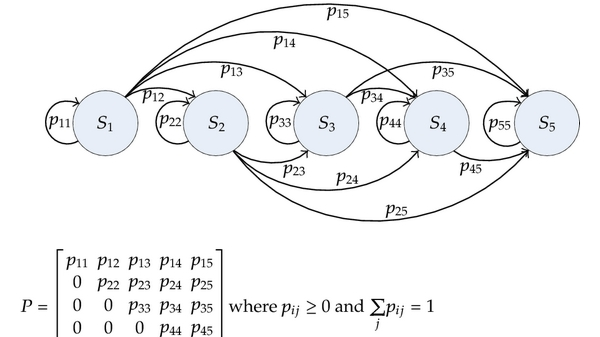
\includegraphics[width=14cm]{markov-chain-example}
	\caption{Example of a Markov Chain}
	\label{ex:markov-chain}
\end{figure}

Here, $P$ is the \textbf{Transition Matrix}. It contains all transition probabilities of the model. A \textbf{Markov Chain} (or Markov Process), is a tuple $(S, P)$, where $S$ is a set of states and $P$ is the transition matrix. A sequence $S_0, ..., S_n$ is called an \textbf{episode}.\\

From this Markov Chain, we can create a \textbf{Markov Reward Process}. This is defined as an extension of the tuple, with the elements $(S, P, R, \gamma)$. $S$ and $P$ mean the same thing as before. However, now we also have a reward function (recall that $R_s = \E[R_{t+1} | S_t=s]$) and a discount factor $\gamma \in [0, 1]$. How to then turn \ref{ex:markov-chain} into a MRP? Simply add reward values to each state in the Markov Chain. The rewards of each state can then be computed with the reward function.\\

Now let's introduce the \textbf{Bellman Equation} for MRP's. It is possible to rewrite the formula of the value function in the following way.

\begin{figure}[h]
	\begin{equation}
		\begin{aligned}
			v(s)&= \E[G_t | S_t = s]\\
				&= \E[R_{t+1} + \gamma (R_{t+2}, \gamma R_{t+3}, ...) | S_t = s]\\
				&= \E[R_{t+1} + \gamma G_{t+1} | S_t = s]\\
				&= \E[R_{t+1} + \gamma v(S_{t+1}) | S_t = s]\\
				&(= R_s + \gamma \sum_{s' \in S} P_{ss'}v(s'))
		\end{aligned}
	\end{equation}
	\caption{Bellman equation of the value function in a MRP}
	\label{form:bellman-value-mrp}
\end{figure}

Now it is possible to see that the value of a state is dependent on the immediate reward, and the return of neighboring states. This can then be computed using the transition matrix ($P_{ss'} > 0 \iff$ you can go from $s$ to $s'$). The bellman equation can then be written in matrix form, namely $v = R + \gamma Pv$.
This can be rewritten as $v = (I - \gamma P)^{-1} R$. This equation can be solved in $O(n^3)$, since a matrix inverse is necessary. For large MRP's, there are several iterative methods to solve this equation. For example,

\begin{itemize}
	\item Dynamic programming
	\item Monte-Carlo evaluation
	\item Temporal-Difference learning
\end{itemize}

These methods will be explained in later chapters.\\

\pagebreak

\section{Markov Decision Processes}

Finally, let's talk about the \textbf{Markov Decision Process}. This is an extension of the MRP, with properties $(S, A, P, R, \gamma)$. It introduces a new set, defining the actions that can be taken. The transition matrix $P^a$ and $R^a$ now also conditionally depend on the action.

\begin{figure}[h]
	\centering
	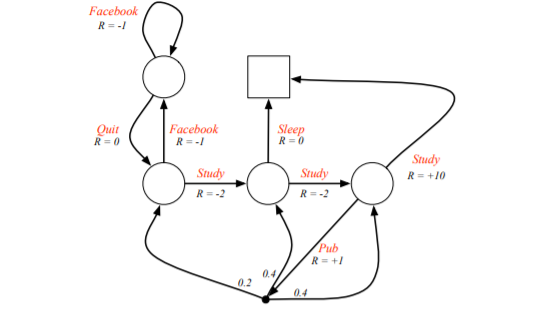
\includegraphics[width=15cm]{mdp-example}
	\caption{Example of a Markov Decision Process}
	\label{ex:mdp}
\end{figure}

\ref{ex:mdp} is an example of a Markov Decision Process. In the image you see that the rewards are now dependent on the actions, as previously explained. Now it is possible to talk about the behavior of an agent. In chapter 1, policies were mentioned. These determine the behavior of agents (like which action to take in which state).\\

Given an MDP and a policy $\pi$. The state sequence $S_0, S_1, ...$ is a Markov Process $(S, P^\pi)$ and the state and reward sequence $S_0, R_1, S_1, R_2, ...$ is a Markov Reward Process $(S, P^\pi, R^\pi, \gamma)$ where $P^\pi_{s, s'} = \sum_{a \in A} \pi(a | s)P^a_{s, s'}$ and $R^\pi_s = \sum_{a \in A} \pi(a | s)R^a_s$ (Law of Total Probability).\\

Similarly to the state-value function $v_\pi(s)$, let's now define the \textbf{action-value} function $q_\pi(s, a) = \E_\pi[G_t | S = s, A = a]$. This is the expected return starting from state s, taking action a, and then following policy $\pi$. In a RL problem, this is what we care about. The goal is to select the best action in a given state, in order to maximize the reward. If we have access to the $q$-values, it is the solution to the problem.\\

After deriving the Bellman equations for the MDP's, we end up with the following formulas.

\begin{figure}[h]
	\begin{equation}
		\begin{aligned}
			v(s)&= \E_\pi[G_t | S_t = s]\\
				&= \E_\pi[R_{t+1} + \gamma v(S_{t+1}) | S_t = s]\\
				&(= \sum_{a \in A}\pi(a|s)q_\pi(s, a))\\
				&(= \sum_{a \in A}\pi(a|s)\left(R^a_s + \gamma \sum_{s' \in S} P^a_{ss'}v_\pi(s')\right))
		\end{aligned}
	\end{equation}
	\caption{Bellman equation of the state value function in a MDP}
	\label{form:bellman-state-value-mdp}
\end{figure}

\begin{figure}[h]
	\begin{equation}
		\begin{aligned}
			q(s, a) &= \E_\pi[G_t | S_t = s, A_t = a]\\
					&= \E_\pi[R_{t+1} + \gamma q(S_{t+1}, A_{t+1}) | S_t = s, A_t = a]\\
					&(= R^a_s + \gamma \sum_{s' \in S} P^a_{ss'}v_\pi(s'))\\	
					&(= R^a_s + \gamma \sum_{s' \in S} P^a_{ss'}\sum_{a' \in A}\pi(a'|s')q_\pi(s', a'))	
		\end{aligned}
	\end{equation}
	\caption{Bellman equation of the action value function in a MDP}
	\label{form:bellman-action-value-mdp}
\end{figure}

The second-last form of formula \eqref{form:bellman-action-value-mdp} can be intuitively thought of as the following. Imagine we are taking a certain action in a state. Then, the environment might bring us into different successor states even if we take the action. So, we have to sum over all these possible successor states and use the law of total probability again to compute the action-values.\\

Now we can talk about optimality. The \textbf{optimal state-value} and \textbf{optimal action-value} functions are defined as $v_*(s) = \max_\pi v_\pi(s)$ and $q_*(s, a) = \max_\pi q_\pi(s, a)$. We can say $\pi \geq \pi'$ if $\forall s: v_\pi(s) \geq v_{\pi'}(s)$. The optimal value function specifies the best possible performance in the MDP. An MDP is "solved" when we know the optimal value. For any MDP, there always exist an optimal policy that is better or equal to all policies. This policy achieves both the optimal value function and the optimal action-value function.\\

An \textbf{optimal policy} can be found by maximizing over $q_*(s, a)$.

\begin{figure}[h]
	\begin{equation}
		\pi_*(a | s) =
		\begin{cases}
			1, & \text{if a = arg$\max_{a \in A} q_*(s, a)$}\\
			0, & \text{otherwise}
		\end{cases}
	\end{equation}
	\caption{Equation for an optimal policy}
	\label{form:optimal-policy}
\end{figure}

Thee optimal value functions are recursively related to the \textbf{Bellman Optimality Equations}. $v_*(s) = \max_a q_*(s, a)$ and $q_*(s, a) = R^a_s + \gamma \sum_{s' \in S} P^a_{ss'}v_*(s')$. Solving for these equations is difficult, since the Bellman Optimality Equation is non-linear. Generally, there is no closed form solution. However, there exist iterative methods to approximate the solution. Example of this are
\begin{itemize}
	\item Value Iteration
	\item Policy Iteration
	\item Q-learning
	\item Sarsa
\end{itemize}

\section{Advanced: Extensions to MDPs}

\subsection{Infinite and continuous MDPs}
\begin{itemize}
	\item Countably infinite state and/or action spaces
	\begin{itemize}
		\item Straightforward
	\end{itemize}
	\item Continuous state and/or action spaces
	\begin{itemize}
		\item Closed form for linear quadratic model (LQR)
	\end{itemize}
	\item Continuous time
	\begin{itemize}
		\item Requires partial differential equations
		\item Hamilton-Jacobi-Bellman (HJB) equation
		\item Limiting case of Bellman equation as time-step approaches 0
	\end{itemize}
\end{itemize}

\subsection{Partially observable MDPs}
A Partially Observable Markov Decision Process is an MDP with hidden states. It is a \textbf{hidden Markov model} with actions. A POMDP is a tuple $(S, A, O, P, R, Z, \gamma)$. We now also have $O$ representing a finite state of observations and $Z$ being an observation function $Z^a_{s'o} = \Prob[O_{t+1} = o | S_{t+1} = s', A_t = a]$.\\

Let's define a \textbf{history} $H_t$ being a sequence of actions, observations and rewards ($H_t = A_0, O_1, R_1, ..., A_{t-1}, O_t, R_t$). A \textbf{belief state} $b(h)$ is a probability distribution over states conditioned on the history h. $b(h) = (\Prob[S_t = s^1 | H_t = h], ..., \Prob[S_t = s^n | H_t = h])$.The history and belief state both satisfy the Markov property. A POMDP can be reduced to an (infinite) history tree and an (infinite) belief state tree.
\let\cleardoublepage\clearpage
\chapter{Planning - Dynamic Programming}

\textbf{Dynamic Programming} (DP) breaks one problem down into smaller sub-problems in order to solve them. Then, you can combine the solutions of the sub-problem to answer the problem.\\

DP is used for planning within an MDP. This means the method assumes there is full knowledge of the MDP. It is technically not Reinforcement Learning yet, since we don't discover an initially unknown environment. It can be used for both \ \textit{prediction} (the input is the MDP and policy, returns value function) and \textit{control} (input only the MDP, returns optimal policy and value function).

\section{Prediction}

\textbf{Iterative policy evaluation} can be used to perform prediction in an MDP (evaluate how good a policy is). On a high level, it works by backing up the Bellman expectation from the states in which rewards are observed. The pseudocode below shows how the algorithm works.

\begin{algorithm}[H]
\caption{Iterative policy evaluation}
\label{alg:it-pol-eval}
    \begin{algorithmic}
    	\REQUIRE the MDP, policy $\pi$
    	\STATE $i \Leftarrow 0$, $v_0(s) \Leftarrow 0$ for each state $s$
        \WHILE{not converged}
        	\FOR{\textbf{each} state $s$}
        		\STATE $v_{i+1}(s) \Leftarrow 
        		\sum_{a \in A} \pi(a|s) \left(R^a_s + \gamma \sum_{s^\prime \in S} P^a_{ss^\prime} v_i(s^\prime) \right)$
        	\ENDFOR
        	\STATE $i \Leftarrow i + 1$
        \ENDWHILE
        \RETURN $v_i$
    \end{algorithmic}
\end{algorithm}

When this algorithm converges, we have obtained the value function $v_\pi$.

\section{Control}

Now that we have a way to evaluate how good a certain policy is, we can start improving it. There are two main ways of performing control using DP. The first method that will be discusses is called \textbf{Policy Iteration}.\\

At each iteration, this method consists of two components: \textbf{policy evaluation} and \textbf{policy improvement}. The whole algorithm works in the following way

\begin{algorithm}[H]
	\caption{Iterative policy evaluation}
	\label{alg:it-pol-eval}
	\begin{algorithmic}
		\REQUIRE the MDP, policy $\pi$
		\WHILE{not converged}
			\STATE $v^\pi \Leftarrow$ iterative policy evaluation with $\pi$
			\STATE $\pi^\prime \Leftarrow greedy(v_\pi)$
			\STATE $\pi = \pi^\prime$
		\ENDWHILE
		\RETURN $v_\pi$, $\pi$
	\end{algorithmic}
\end{algorithm}

The image below shows how this algorithm works on a higher level.

\begin{figure}[H]
	\centering
	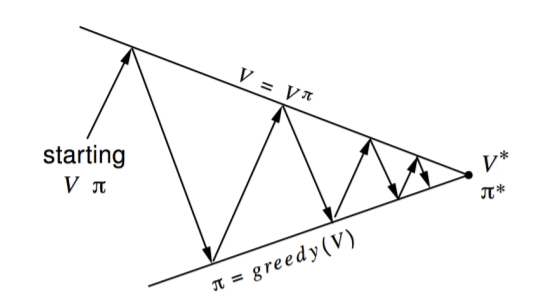
\includegraphics[width=8cm]{policy-iteration}
	\caption{Policy Iteration}
	\label{img:policy-iteration}
\end{figure}

Why does acting greedily with respect to the obtained $v_\pi$ improve the policy? There is a relatively simple proof for this. Say we choose a deterministic policy $\pi(s)$. Acting greedily would mean we create a new policy $\pi^\prime(s) = \arg \max_{a \in A} q_\pi(s, a)$. This means that $q_\pi(s, \pi^\prime(s)) = \max_{a \in A} q_\pi(s,a) \geq q_\pi(s, \pi(s)) = v_\pi(s)$. So we know $q_\pi(s, \pi^\prime(s)) \geq v_\pi(s)$. Therefore, $v_{\pi^\prime}(s) \geq v_\pi(s)$.\\

This means if the improvement stops, we must have satisfied the Bellman optimality equation.\\

Policy iteration can be generalized. Before we performed policy evaluation until we obtained $v_\pi$. However, this is not necessary. The next DP control algorithm, \textbf{Value Iteration}, is a special variant of policy iteration, updating the policy after every step (so not after it converges to $v_\pi$). You can basically use \textbf{any} policy evaluation and policy improvement algorithm to perform policy iteration.\\

Lets now start talking about Value Iteration. This method works because of the \textit{Principle of Optimality}, which states the following: An optimal policy can be subdivided into two components

\begin{itemize}
	\item An optimal first action $A_*$
	\item An optimal policy from successor state $S^\prime$
\end{itemize}

This means that if we know the solution to $v_*(s^\prime)$, we can find $v_*(s)$ by performing the following one-step lookahead. This is possible due to the Bellman optimality equations.

\begin{equation*}
		v^*(s) = \max_{a \in A} \left( R^a_s + \gamma \sum_{s^\prime \in S} P^a_{ss^\prime} v_*(s^\prime)\right)
\end{equation*}

The intuition is that you can start with the final rewards and work your way backwards. 

\begin{algorithm}[H]
	\caption{Value iteration}
	\label{alg:val-iter}
	\begin{algorithmic}
		\REQUIRE the MDP
		\STATE $i \Leftarrow 0$, $v_0(s) \Leftarrow 0$ for each state $s$
		\WHILE{not converged}
			\FOR{\textbf{each} state $s$}
				\STATE $v_{i+1}(s) \Leftarrow 
				\max_{a \in A} \left(R^a_s + \gamma \sum_{s^\prime \in S} P^a_{ss^\prime} v_i(s^\prime)\right)$
			\ENDFOR
			\STATE $i \Leftarrow i + 1$
		\ENDWHILE
		\STATE $v_* \Leftarrow v_i, \pi_*(s) \Leftarrow \arg\max_{a \in A} R^a_s + \gamma\sum_{s' \in S} P^a_{ss'}v_*(s')$
		\RETURN $v_*, \pi_*$
	\end{algorithmic}
\end{algorithm}

Observe that the policy is extracted by acting greedily with respect to the computed q-values for any state. For any intermediate value functions, this might not be true. These in-between value function might not correspond to any policy.\\

The previously discusses algorithms all share a runtime complexity of $O(n^2m)$ per iteration when computing $v$, $n$ being the number of states and $m$ the number of actions. However, the same process can be applied to compute the q-values. This would be $O(n^2m^2)$ per iteration.

\section{Extensions to DP}

So far all described DP methods are \textit{synchronous}. This means all states are updated in parallel. However, these algorithms can also be implemented in an \textit{asynchronous} manner. Since it uses more updated information, it generally converges a lot faster than the synchronous variant. It is also guaranteed to converge as long as all states are continued to be visited. The following three ideas are simple ideas for asynchronous DP with Value Iteration.

\begin{itemize}
	\item In-place DP
	
	Instead of using different value functions $v_i$ at each iteration, we only use one value function. $v_{i+1}(s) = \max_{a \in A} \left(R^a_s + \gamma \sum_{s^\prime \in S} P^a_{ss^\prime} v_i(s^\prime)\right)$ will then become $v(s) = \max_{a \in A} \left(R^a_s + \gamma \sum_{s^\prime \in S} P^a_{ss^\prime} v(s^\prime)\right)$.
	
	\item Prioritized sweeping
	
	Instead of iterating over all states in one order, it is possible to use the magnitude of Bellman error to guide the selection of the next state to evaluate. This bellman error can be expressed as 
	
	\begin{equation*}
		\left|\max_{a \in A} \left(R^a_s + \gamma \sum_{s' \in S} P^a_{ss'}v(s')\right) - v(s)\right|
	\end{equation*}

	The idea is to backup the state with the largest remaining Bellman error and update the Bellman error of the affected states after. This requires knowledge of the reverse dynamics of the MDP, since we are working backwards. It can be very simply implemented using a priority queue.
	
	\item Real-time DP
	
	The idea here is to only update states that are relevant to the agent. The agent's experience can guide the state selection. So, after each time step, we observe $S_t, A_t$ and $R_{t+1}$. We back-up the state $S_t$ by $v(S_t) = \max_{a \in A} \left(R^a_{S_t} + \gamma \sum_{s^\prime \in S} P^a_{S_{t}s^\prime} v(s^\prime)\right)$.
	
\end{itemize}

The DP approach that was discussed this chapter is already good. It is effective for problems containing millions of states. However, since it uses full-width backups, each successor state and action is considered. For large problems this causes DP to suffer from the curse of dimensionality; the number of states grow exponentially with the number of state variables. As proposed in further chapters, this problem is approached using sample backups.

%TODO: Add something about algorithm convergance
\let\cleardoublepage\clearpage
\chapter{Model-Free Prediction}

Last chapter was about planning by dynamic programming. This was an approach to solving a known MDP. In many cases, however, we do not have access to the full MDP. In this case, we are talking about unknown MDPs. In this chapter, estimating the value function of an unknown MDP will be discussed.

\section{Monte-Carlo RL}

Sampling methods like Monte-Carlo methods are about learning from episodes of experience. This means they don't need to have any knowledge of the dynamics of the MDP (transitions and rewards). This makes them model-free methods. The point of MC methods is to run until the end of each episode. This means it can only work if episodes always terminate. It backtracks the experience that was generated during the episode to estimate the value function. They are based on one simple idea: \textbf{value = mean return}.\\

Walking through episodes of a problem using policy $\pi$ yields the information $S_1, A_1, R_1, ..., S_k \sim \pi$. The return is the total discounted reward, computed by $G_t = R_{t+1} + \gamma R_{t+2} + ... + \gamma^{T-1}R_T$. Then, $v_\pi(s) = \E_\pi \left[G_t | S_t = s\right]$. Instead of this \textit{expected} return, MC policy evaluation uses an \textit{empirical mean} return.\\

\begin{algorithm}[H]
	\caption{Iteration in Monte-Carlo methods}
	\label{alg:MC-eval}
	\begin{algorithmic}
		\REQUIRE policy $\pi$
		\STATE $\forall s: V(s) \Leftarrow 0, N(s) \Leftarrow 0, S(s) \Leftarrow 0$
		\FOR{$t \Leftarrow 0, ..., T$}
			\STATE $A_t, R_{t+1}, S_{t+1} \sim \pi$
			\STATE $N(S_t) \Leftarrow N(S_t) + 1$
			\STATE $S(S_t) \Leftarrow S(S_t) + G_t$
			\STATE $V(S_t) \Leftarrow \frac{S(S_t)}{N(S_t)}$
		\ENDFOR
		\RETURN $V$
	\end{algorithmic}
\end{algorithm}

By the law of large numbers
\begin{equation*}
	\lim_{N(s) \Rightarrow \infty} V(s) = v_\pi(s)
\end{equation*} 

This algorithm uses an \textit{every-visit} approach, meaning it will execute an iteration every time $S_t$ has been encountered in an episode. There is a second approach called \textit{first-visit}. This works by only doing the iteration for state $S_t$ at most once per episode, when it is encountered for the first time. 

Imagine that at time $t$ you observe $S_t$, but the same state is observed at time $t+2$. Then, $S_t = S_{t+2}$. The first-visit approach will not do the iteration at $t+2$, but the every visit will.\\

There is also a way of computing the mean incrementally.
\begin{equation*}
	\begin{aligned}
		V_t(S) & = \frac{S_t(S)}{N_t(S)}\\
			 & = \frac{1}{N_t(S)} (G_t + S_{t-1}(S))\\
			 & = \frac{1}{N_t(S)} (G_t + (N_t(S)-1)V_{t-1}(S))\\
			 & = V_{t-1}(S) + \frac{1}{N_t(S)} (G_t - V_{t-1}(S))\\
		V(S_t) & = V(S_t) + \frac{1}{N(S_t)} (G_t - V(S_t)) 
	\end{aligned}
\end{equation*}

This way you can see how it works intuitively. The current perception of the value is updated using a difference in the observed return and current perception of the value, weighted by the number of times a state is visited.\\

However, this means that we will never completely forget old experience, since we are using this moving average. In non-stationary problems, it may be useful to track the running mean to forget old episodes. This can be achieved by for example replacing $\frac{1}{N(S_t)}$ by a constant $\alpha$. The new equation will become $V(S_t) = V(S_t) + \alpha (G_t - V(S_t))$.

\section{Temporal-Difference RL}

One problem with Monte-Carlo methods is that we need episodes to terminate. TD-Learning on the other hand, does not need this. Like MC, they learn directly from episodes of experience. They are also model-free. The key difference is that TD-Learning uses a concept called \textbf{bootstrapping} to learn from incomplete episodes. They basically update towards a guess of $G_t$.\\

The simplest TD-algorithm is called TD(0). It attempts to update the value towards the estimated return $R_{t+1} + \gamma V(S_{t+1})$, which it uses as a guess for the expected return $G_t$. This value is often referred to as the TD target. Updating the value function will then become $V(S_t) = V(S_t) + \alpha (R_{t+1} + \gamma V(S_{t+1}) - V(S_t)) = V(S_t) + \alpha \delta_t$ where $\delta_t$ is referred to  as the TD error.

\section{Comparison of methods}

One big difference between TD and MC is that TD can learn \textit{online} after every step and without the final outcome. MC must wait until the episode is over, not being able to learn from incomplete/non-terminating sequences.

We know that the return $G_t = R_{t+1} + \gamma V_\pi(S_{t+1})$ is an \textit{unbiased} estimate of $v_\pi(S_t)$. TD uses a \textit{biased} estimate of the value function, since it uses $R_{t+1} + \gamma V(S_{t+1})$ to bootstrap. The positive thing about this is that the TD target has a much lower variance than the return. This is because the return depends on many random actions/transitions/rewards, while the TD target only depends on one random action/transition/reward.

Both MC and TD converge to the true value function for a policy as we get infinite experience. However, for finite batches of experience that are repeatedly sampled, they will not produce the same results.

Monte-Carlo methods converge to the solution to the best fit of the observed return. It has the objective function
\begin{equation*}
	\min \sum_{k = 1}^K \sum_{t = 1}^{T_k} (G_t^k - V(s_t^k))^2
\end{equation*}

Temporal-Difference methods on the other hand converge to the solution of the \textit{maximum likelihood Markov model}. It constructs and solves (given $\pi$) the MDP $(S, A, \hat{P}, \hat{R}, \gamma)$ that best fits the data.
\begin{equation*}
	\begin{aligned}
		& \hat{P^a_{ss'}} = \frac{1}{N(s,a)} \sum_{k = 1}^K \sum_{t = 1}^{T_k} 1(s^k_t, a^k_t, s^k_{t+1} = s, a, s')\\
		& \hat{R^a_{s}} = \frac{1}{N(s,a)} \sum_{k = 1}^K \sum_{t = 1}^{T_k} 1(s^k_t, a^k_t = s, a)r^k_t
	\end{aligned}
\end{equation*}

From this you can see TD exploits the Markov property. Standard MC does not do this. For this reason, TD is usually more effective in Markov environments and MC in non-Markov environments.

\section{TD($\lambda$)}

As we saw before, TD(0) looks one step into the future, by calculating $R_{t+1} + \gamma V(S_{t+1})$. Can we look more steps into the future? The answer is yes. For example, a 2-step TD target can be calculated as $R_{t+1} + \gamma R_{t+2} + \gamma^2 V(S_{t+2})$. It is interesting to notice that when we look $\infty$ steps into the future, we converge to the Monte-Carlo method!

In general, the $n$-step return $G^{(n)}_t = R_{t+1} + \gamma R_{t+2} + ... + \gamma^{n-1} R_{t+n} + \gamma^n V(S_{t+n})$. To perform $n$-step TD, you just use $G^{(n)}_t$ as your estimation of $G_t$.\\

We can even average different $n$-step returns to create a more sound estimate of $G_t$. For example, $\frac{1}{2} G^{(2)} + \frac{1}{2} G^{(4)}$. The idea that rises is whether we can efficiently combine information from all time-steps.\\

This is actually what TD($\lambda$) does. It defines the $\lambda$-return $G^\lambda_t$ that combines all $n$-step returns. The method uses weighting $(1 - \lambda)\lambda^{n - 1}$. The reason for this weighting is that it has nice convergence properties that allow us to calculate this return in the same time-complexity as TD(0).

We obtain $G^\lambda_t = (1-\lambda) \sum^\infty_{n = 1} \lambda^{n-1} G_t^{(n)}$. \textbf{Forward view TD($\lambda$)} will then be $V(S_t) = V(S_t) + \alpha (G^\lambda_t - V(S_t))$.

\begin{figure}[H]
	\centering
	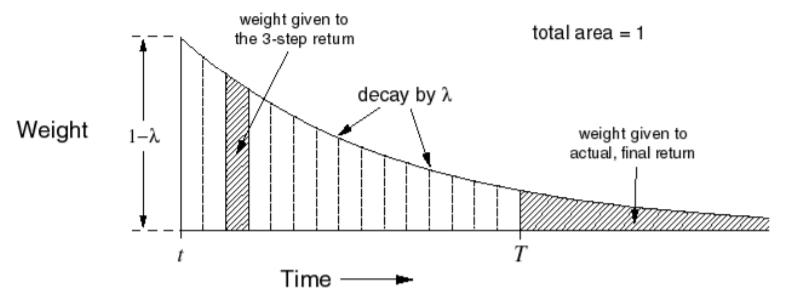
\includegraphics[width=14cm]{lambda-weighting}
	\caption{Influence of weighting on different returns $G^{(n)}$}
	\label{fig:lambda-weighting}
\end{figure}

As seen in \ref{fig:lambda-weighting}, more recent states get a higher weighting in TD($\lambda$). The weight decays as we look more into the future.\\

There is a problem with this forward-view algorithm. Just like MC, the estimated return can only be computed once the episode terminates. Luckily, there is another view for TD($\lambda$) called the \textbf{Backward View}. This algorithm allows for updating online, on every step from incomplete sequences. \\

To understand Backward View TD, lets introduce a concept called \textbf{Eligibility traces}. Imagine you're in a situation where you just got electrocuted. This happened right before you heard a bell right. Before that bell even rang, light flashed three times. What do you think caused the shock? The light flashes or the bell? 

The idea of this is that this is controlled by \textbf{Frequency heuristics} and \textbf{Recency heuristics}. We can combine both of these heuristics to form Eligibility Traces. Let $E_t(S)$ be the eligibility trace of state $s$ at time $t$. Initially, $E_0(s) = 0$. We create the recursive relationship $E_t(s) = \gamma \lambda E_{t-1}(s) + 1(S_t = s)$. Observe that at time $t$, if we're in state $s$, a value of 1 will be added to $E_t(s)$. However, for all other previously visited states, their trace only gets decayed. This corresponds to the intuition of figure \ref{fig:lambda-weighting}.\\

For Backward View TD($\lambda$), the idea is the following
\begin{itemize}
	\item Keep an eligibility trace for all states $s$
	\item Update value V(s) for every state $s$
	\item In proportion to TD-error $\delta_t$ and $E_t(s)$, we say $V(s) = V(s) + \alpha \delta_t E_t(s)$
\end{itemize}

Intuitively, this means you are constantly decaying and updating the values of previously observed states. When $\lambda = 0$, we end up with TD(0). When $\lambda = 1$, the credit is deferred until the end of the episode. This means that \textit{over the course of an episode}, the total update for TD(1) is the same as the total update for every-visit MC.

\begin{algorithm}[H]
	\caption{Iteration of TD($\lambda$)}
	\label{alg:MC-eval}
	\begin{algorithmic}
		\REQUIRE policy $\pi$
		\STATE $\forall s: V(s) \Leftarrow 0, E(s) = 0$
		\FOR{$t \Leftarrow 0, ..., T$}
		\STATE $A_t, R_{t+1}, S_{t+1} \sim \pi$
		\STATE $\delta_t \Leftarrow R_{t+1} + \gamma V(S_{t+1}) - V(S_t)$
		\STATE $E(S_t) \Leftarrow E(S_t) + 1$
			\FOR{all unique previously occurred $s$}
				\STATE $V(s) \Leftarrow V(s) + \alpha \delta_t E(s)$
				\STATE $E(s) \Leftarrow \gamma \lambda E(s)$
			\ENDFOR
		\ENDFOR
		\RETURN $V$
	\end{algorithmic}
\end{algorithm}
 
\let\cleardoublepage\clearpage
\chapter{Model-Free Control}

This chapter several methods for Model-Free control will be discussed. Algorithms like Monte-Carlo and Temporal-Difference learning are often used for prediction, but how can these concepts be used for control? There are two different ways of learning when sampling, these are 

\begin{itemize}
	\item \textbf{On-policy} learning
	
	The goal is to learn about policy $\pi$ from experience that is being sampled by $\pi$
	
	\item \textbf{Off-policy} learning
	
	The goal is to learn about policy $\pi$ from experience that is being sampled by a policy $\mu$, $\mu \neq \pi$.
\end{itemize}

From generalized policy iteration, any valid \textit{policy evaluation} algorithm can be followed by any valid \textit{policy improvement} algorithm and iterated in order to find the optimal policy. The first question that should come up in your mind is "Can we just use the algorithms from the previous chapter for the policy evaluation step?". Initially, there are two problems with this.

\begin{enumerate}
	\item Greedy policy improvement over $V(s)$ requires a model of the MDP, since $\pi'(s) = \arg\max_{a \in A} R^a_s + P^a_{ss'} V(s')$. We do not have access to the rewards and the transition probabilities.
	
	We know this is equal to $\pi'(s) = \arg\max_{a \in A} Q(s,a)$. So learning the q-value function instead of the value function will be \textit{model-free}.
	
	\item Being greedy using sampling methods does not ensure we cover the entire state space.
	
	Exploration vs. exploitation is a whole problem on its own in Reinforcement Learning, that will be discussed in a later chapter. For now we can consider the easiest way to ensure continual exploration. Instead of being greedy, lets be \textbf{$\epsilon$-greedy}. The policy becomes the following
	
	\begin{equation}
		\pi(a | s) = \begin{cases}
			\epsilon/m + 1 - \epsilon, & a^* = \arg\max_{a \in A} Q(s, a)\\
			\epsilon/m, & \text{otherwise}.
		\end{cases}
	\end{equation}

	This means that there is a $1 - \epsilon$ probability to choose the greedy action and an $\epsilon$ probability to choose any other random action, wtih $m$ being the number of actions.\\
	
	Now, all that is left to be done is prove any $\epsilon$-greedy policy $\pi'$ with respect to $q_\pi$ actually is an improvement to $\pi$. The proof is rather simple:
	
	\begin{equation*}
		\begin{aligned}
			q_\pi(s, \pi'(s)) & = \sum_{a \in A} \pi'(a | s) q_\pi(s, a)\\
							  & = \epsilon/m \sum_{a \in A} q_\pi(s, a) + (1 - \epsilon) \max_{a \in A} q_\pi(s, a)\\
							  & \geq \epsilon/m \sum_{a \in A} q_\pi(s, a) + (1 - \epsilon) \sum_{a \in A} \frac{\pi(a|s) - \epsilon/m}{1 - \epsilon} q_\pi(s, a)\\
							  & = \sum_{a \in A} \pi(a|s) q_\pi(s, a) = v_\pi(s)
		\end{aligned}
	\end{equation*}

	Then, from policy improvement theorem, $v_{\pi'}(s) \geq v_\pi(s)$.
\end{enumerate}

We have now tackled the problems that prevented us to use the idea of generalized policy iteration. The methods we have previously seen can now be applied to solve the problem.

\section{On-Policy methods}

Last chapter Monte-Carlo and TD-Learning were discussed for policy evaluation. This section will show how to apply these algorithms for control tasks.

\subsection{Monte-Carlo Control}

\begin{figure}[H]
	\centering
	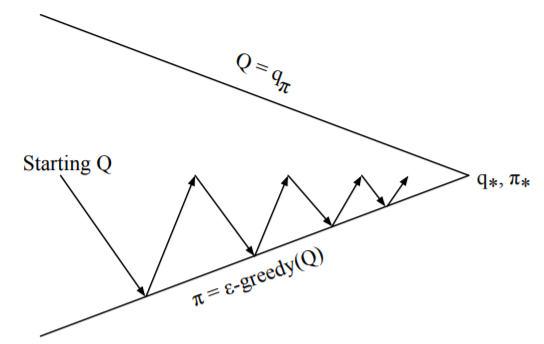
\includegraphics[width=9cm]{MC-Control}
	\caption{Monte-Carlo Control algorithm}
	\label{fig:MC-control}
\end{figure}

The idea of \ref{fig:MC-control} is similar to policy iteration. In order to speed up convergence, it is not necessary to evaluate the policy until $q_\pi$ is obtained. A better approach is to perform Monte-Carlo policy evaluation \ref{alg:MC-eval} until the end of the episode, and then perform an $\epsilon$-greedy policy improvement step with respect to the computed q-values.\\

There is a theorem called \textit{Greedy in the Limit with Infinite Exploration} (GLIE), which ensures you converge to the optimal policy (which is always greedy). The following two rules must apply
\begin{enumerate}
	\item $\lim_{k \Rightarrow \infty} N_k(s, a) = \infty$
	\item $\lim_{k \Rightarrow \infty} \pi_k(a|s) = 1(a = \arg\max_{a' \in A} Q_k(s, a'))$
\end{enumerate}
Here, the $\epsilon$-greedy policy would reduce to greedy when there is infinite experience. For example, $\epsilon$-greedy is GLIE if $\epsilon$ reduces to zero at the rate $\epsilon_k = \frac{1}{k}$. Lets construct an algorithm based on this knowledge.

\begin{algorithm}[H]
	\caption{One iteration of GLIE Monte-Carlo Control}
	\label{alg:GLIE-MC-Control}
	\begin{algorithmic}
		\FOR{$t \Leftarrow 0, ..., T$}
			\STATE $A_t, R_{t+1}, S_{t+1} \sim \pi$
			\STATE $N(S_t, A_t) \Leftarrow N(S_t, A_t) + 1$
			\STATE $Q(S_t, A_t) \Leftarrow Q(S_t, A_t) + \frac{1}{N(S_t, A_t)} (G_t - Q(S_t, A_t))$
		\ENDFOR
		\STATE $\epsilon \Leftarrow 1/k, \pi \Leftarrow \epsilon$-greedy($Q$)
		\RETURN $Q, \pi$
	\end{algorithmic}
\end{algorithm}

\subsection{TD-Control (SARSA)}

TD-Learning has several advantages over MC such as a lower variance, online updating, and being able to learn from incomplete sequences. It would be a natural idea to use TD instead of MC in the control loop that was previously presented. This method is referred to as \textbf{SARSA}. This yields the following algorithm

\begin{algorithm}[H]
	\caption{One iteration of SARSA}
	\label{alg:SARSA}
	\begin{algorithmic}
		\REQUIRE $\pi \Leftarrow \epsilon$-greedy($Q$)
		\FOR{$t \Leftarrow 0, ..., T$}
		\STATE $A_t, R_{t+1}, S_{t+1}, A_{t+1} \sim \pi$
		\STATE $Q(S_t, A_t) \Leftarrow Q(S_t, A_t) + \alpha \left[R_{t+1} + \gamma Q(S_{t+1}, A_{t+1}) - Q(S_t, A_t) \right]$
		\ENDFOR
		\STATE $\epsilon \Leftarrow 1/k, \pi \Leftarrow \epsilon$-greedy($Q$)
		\RETURN $Q, \pi$
	\end{algorithmic}
\end{algorithm}

SARSA converges to the optimal action-value function under the following conditions:
\begin{enumerate}
	\item GLIE sequence of policies $\pi_t(a|s)$
	\item \textbf{Robbins-Monro} sequence of step-sizes $\alpha_t$ ($\sum_{t = 1}^\infty \alpha_t = \infty$ and $\sum_{t = 1}^\infty \alpha_t^2 < \infty$)
\end{enumerate}
In practice however, this is only very rarely taken into account (like with a constraint learning rate $\alpha$). It does not seem to pose that much of a threat. 

Just like $n$-step TD and TD($\lambda$), there exists \textbf{n-step SARSA} and \textbf{SARSA($\lambda$)}. SARSA($\lambda$) also has the same forward- and backward-view algorithms. These are the exact same concepts. The only difference is SARSA is for action-values. For this reason, I will just give you the formulas for it. The intuition is the same as in the previous chapter.
\begin{enumerate}
	\item $n$-step SARSA\\
	
	$Q(S_t, A_t) = Q(S_t, A_t) + \alpha \left[q_t^{(n)} - Q(S_t, A_t) \right]$\\
	$q_t^{(n)} = R_{t+1} + \gamma R_{t+2} + ... + \gamma^{n-1} R_{t+n} + \gamma^n Q(S_{t+n}, A_{t+n})$
	
	\item (Forward View) SARSA($\lambda$)
	
	$Q(S_t, A_t) = Q(S_t, A_t) + \alpha \left[q_t^\lambda - Q(S_t, A_t) \right]$\\
	$q_t^\lambda = (1-\lambda) \sum_{n = 1}^\infty \lambda^{n-1} q_t^{(n)}$	
\end{enumerate}

\begin{algorithm}[H]
	\caption{Iteration of (backward view) SARSA($\lambda$)}
	\label{alg:MC-eval}
	\begin{algorithmic}
		\REQUIRE $\pi \Leftarrow \epsilon$-greedy($Q$), $Q$
		\STATE $E(s, a) = 0$
		\STATE Initialize $S_0, A_0$
		\FOR{$t \Leftarrow 0, ..., T$}
		\STATE $R_{t+1}, S_{t+1}, A_{t+1} \sim \pi$
		\STATE $\delta_t \Leftarrow R_{t+1} + \gamma Q(S_{t+1}, A_{t+1}) - Q(S_t, A_t)$
		\STATE $E(S_t, A_t) \Leftarrow E(S_t, A_t) + 1$
		\FOR{all unique previously occurred $(s, a)$ pairs}
		\STATE $Q(s, a) \Leftarrow Q(s, a) + \alpha \delta_t E(s, a)$
		\STATE $E(s, a) \Leftarrow \gamma \lambda E(s, a)$
		\ENDFOR
		\ENDFOR
		\RETURN $V$
	\end{algorithmic}
\end{algorithm}

The eligibility traces for the backward view algorithm are, just like the value function, now taken into account for all state-action pairs.

\begin{figure}[H]
	\centering
	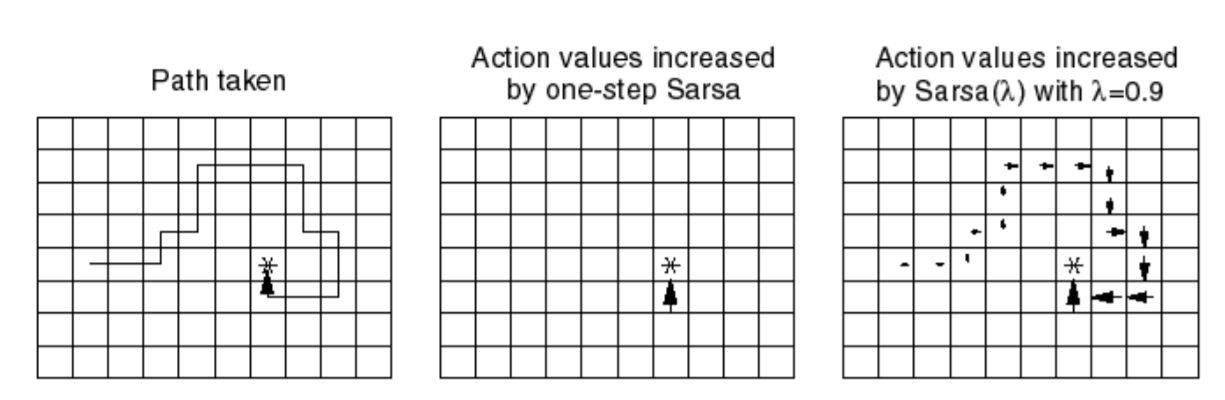
\includegraphics[width=12cm]{lambda-role-sarsa}
	\caption{The role of $\lambda$ in SARSA($\lambda$)}
	\label{fig:lambda-sarsa-role}
\end{figure}

In \ref{fig:lambda-sarsa-role}, you can see the role of the lambda parameter. When receiving reward (in the image only at the end), the combination of the recency and visitation heuristic made into the eligibility trace makes sure there is a decay in propagating the reward backwards. This is all one iteration of the algorithm.

\section{Off-Policy methods}

The goal of off-policy learning is to evaluate the target policy $\pi(a|s)$ to compute $v_\pi(s)$ or $q_\pi(s, a)$. All of this happens while following a different policy $\mu(a|s)$. This is referred to as the \textit{behaviour policy}. The most well-known use of this is learning about the optimal policy while following a \textit{exploratory} policy.

\textbf{Importance Sampling} is a way of estimating the expectation of a different distribution. The underlying idea is the following
\begin{equation*}
	\begin{aligned}
		\E_{X \sim P} \left[f(X)\right] & = \sum f(X) P(x)
										& = \sum f(X)\frac{P(X)}{Q(X)} Q(X)
										& = \E_{X \sim Q} \left[f(X) \frac{P(X)}{Q(X)}\right]
	\end{aligned}
\end{equation*}
From this derivation, notice that it is possible to estimate the expectation of sampling distribution $P$ while sampling from $Q$, using a simple division $\frac{P(X)}{Q(X)}$.

\subsection{Importance Sampling for Off-Policy MC / TD}

The idea of this simple division can be used in the Monte-Carlo return and TD target. This means we could follow policy $\mu$, while learning policy $\pi$ by just dividing $\pi$ by $\mu$ for every time-step (as seen in the proof).
\begin{equation*}
	G_t^{\pi/\mu} = \frac{\pi(A_t|S_t)}{\mu(A_t|S_t)} \frac{\pi(A_t+1|S_t+1)}{\mu(A_t+1|S_t+1)} ... \frac{\pi(A_T|S_T)}{\mu(A_T|S_T)} G_t
\end{equation*} 

The value will then be updated towards the corrected return: $V_{k+1}(S_t) = V_k(S_t) + \alpha \left(G_t^{\pi/\mu} - V_k(S_t)\right)$. There are several downsides to using this method. The first one is that it can not be used if $\mu = 0, \pi \neq 0$. More importantly, it can dramatically increase variance. This is of course something to avoid when possible.

For TD, the update rule becomes

\begin{equation*}
	V_{k+1}(S_t) = V_k(S_t) + \alpha \left(\frac{\pi(A_t|S_t)}{\mu(A_t|S_t)} (R_{t+1} + \gamma V_k(S_{t+1})) - V_k(S_t)\right)
\end{equation*}

The benefit to this is that it will have a much lower variance than the MC approach. It means the policies only need to be similar over a single step instead of the whole episode chain.

\subsection{Q-Learning}

Now lets consider off-policy learning for action-values $Q(s, a)$. The idea of \textbf{Q-Learning} is to choose the next action using a behaviour policy $A_{t+1} \sim \mu(.|S_t)$, but an alternative successor action $A' \sim \pi(.|S_t)$ is also considered. $Q(S_t, A_t)$ will then be updated towards the value of the alternative action. $Q_{k+1}(S_t, A_t) = Q_k(S_t, A_t) + \alpha \left(R_{t+1} + \gamma Q_k(S_{t+1}, A') - Q_k(S_t, A_t)\right)$.

Now allow both policies to be able to improve. $\pi(S_{t+1}) = \arg\max_{a'} Q(S_{t+1}, a')$ and $\mu = \epsilon$-greedy($Q$). In this case, the Q-learning target simplifies to the following

\begin{equation}
	\begin{aligned}
		  & R_{t+1} + \gamma Q(S_{t+1}, A')\\
		= & R_{t+1} + \gamma Q(S_{t+1}, \arg\max_{a'} Q(S_t, a'))\\
		= & R_{t+1} + \gamma \max_{a'} Q(S_{t+1}, a')
	\end{aligned}
\end{equation}

The algorithm of Q-Learning is then

\begin{algorithm}[H]
	\caption{One iteration of Q-Learning}
	\label{alg:Q-Learning}
	\begin{algorithmic}
		\REQUIRE $\pi \Leftarrow \epsilon$-greedy($Q$)$, Q$
		\FOR{$t \Leftarrow 0, ..., T$}
		\STATE $A_t, R_{t+1}, S_{t+1}, A_{t+1} \sim \pi$
		\STATE $Q(S_t, A_t) \Leftarrow Q(S_t, A_t) + \alpha \left[R_{t+1} + \gamma \max_{A_{t+1}} Q(S_{t+1}, A_{t+1}) - Q(S_t, A_t) \right]$
		\ENDFOR
		\RETURN $Q, \pi$
	\end{algorithmic}
\end{algorithm}
\let\cleardoublepage\clearpage
\chapter{Value Function Approximation}

Before this lecture, the value function was always defined per state. But what if the problems are really big? The game of Go for example has $10^{170}$ states. Some problems even have a \textit{continuous} state space. How is it possible to scale up the previously discussed model-free methods for prediction and control to handle these situations?

The whole time, (action-)value functions were represented using a \textit{lookup table}, where each state had a corresponding value. The problem with large MDP's is that it is too slow to learn the value for each state individually, or even impossible to store all states or actions in memory.

The solution that will be proposed is to estimate the value function using \textbf{function approximation}. This means we use parameters $w$ estimate the value functions $\hat{v}(s, w) \approx v_\pi(s)$ or $\hat{q}(s, a, w) \approx q_\pi(s, a)$. There is a really nice benefit to this. After learning $w$ (using for example MC or TD learning), it will also be able to \textit{generalize} to unseen states.

This chapter will focus on \textit{differentiable} function approximators, since they can be updated using gradient-based optimization. Furthermore, the method must be able to handle \textit{non-stationary} and \textit{non-iid} data.

Two different methods of learning will be discussed, incremental methods and batch methods.

\section{Incremental Methods}

This book assumes you are already familiar with the concept of \textbf{Gradient Descent}. If you are not, here is a quick explanation. If $J(w)$ is a differentiable function of parameter vector $w$. The idea is to update the parameters in the direction of the gradient. We obtain $w = w - \alpha \nabla_w J(w)$ where $\alpha$ is a step-size parameter.

The goal of \textit{Value-function approximation} using Stochastic Gradient Descent (SGD), is to find the parameter vector $w$ in order to minimize the mean-squared error between the approximate value $\hat{v}(s, w)$ and $v_\pi(s)$. The cost function to minimize is then $J(w) = \E_\pi \left[(v_\pi(S) - \hat{v}(S, w))^2\right]$.

Gradient descent converges to a \textit{local} minimum. SGD will do this by sampling the gradient based on one single sample. The expected update is then equal to the full gradient update.

\subsection{Prediction algorithms}

The state of the problem can be represented by a \textbf{feature vector} $x(S)$, where each element is a feature that described the state (preferably independently). The value function is equal to $\hat{v}(S, w) = x(S)^\intercal w$.

Table-lookup is actually a special case of linear function approximation. If a state is a one-hot-encoding of all states, then the dot product with parameter vector $w$ is just $v(S_i) = w_i$.

Since it is impossible to use the true value function $v_\pi$ in the cost function, lets substitute in the targets instead. These are $G_t$ for MC and $G^\lambda_t$ for TD($\lambda$). The following are more detailed descriptions for these methods

\begin{itemize}
	\item \textbf{MC}
	
	Return $G_t$ is an unbiased, noisy sample of $v_\pi(S_t)$. For that reason, it is possible to apply supervised learning to the data $(S_1, G_1), (S_2, G_2), ..., (S_T, G_T)$. $\Delta w = \alpha (G_t - \hat{v}(S_t, w)) \nabla_w \hat{v}(S_t, w) = \alpha (G_t - \hat{v}(S_t, w)) x(S_t)$. Monte-carlo evaluation converges to a local optimum, even when using non-linear function approximation.
	
	\item \textbf{TD(0)}
		
	Return $R_{t+1} + \gamma \hat{v}(S_{t+1}, w)$ is a biased sample of $v_\pi(S_t)$. It is possible to apply supervised learning to the data $(S_1, R_2 + \gamma \hat{v}(S_2, w)), (S_2, R_3 + \gamma \hat{v}(S_3, w)), ..., (S_{T-1}, R_T)$. $\Delta w = \alpha (R_{t+1} + \gamma \hat{v}(S_{t+1}, w) - \hat{v}(S_t, w)) x(S_t)$. Linear TD(0) converges close to the global optimum.
	
	\item \textbf{TD($\lambda$)}
	
	Return $G^\lambda_t$ is also a biased sample of $v_\pi(S_t)$. It is again possible to apply supervised learning to the data $(S_1, G^\lambda_1), (S_2, G^\lambda_2), ..., (S_{T-1}, G^\lambda_{T-1})$. 
	
	\begin{itemize}
		\item Forward view linear TD($\lambda$)
		
		\begin{equation*}
			\Delta w = \alpha (G^\lambda_t - \hat{v}(S_t, w)) x(S_t)
		\end{equation*}
			
		\item Backward view linear TD($\lambda$)
		
		\begin{equation*}
			\begin{aligned}
				\delta_t & = R_{t+1} + \gamma \hat{v}(S_{t+1}, w) - \hat{v}(S_t, w)\\
				E_t 	 & = \gamma \lambda E_{t-1} + \hat{v}(S_t, w)\\
				\Delta w & = \alpha \delta_t E_t
			\end{aligned}
		\end{equation*}
		
		Here, the eligibility traces are defined for every parameter in the function approximator.
				
	\end{itemize}
	The forward and backward view of linear TD($\lambda$) are again equivalent.
\end{itemize}

\subsection{Control algorithms}

Control, just like prediction, preserves the same intuition from its tabular case. First, \textit{approximate} policy evaluation ($\hat{q}(., ., w) \approx q_\pi$) will be performed, followed by an $\epsilon$-greedy policy improvement. The goal becomes to minimize the following cost function: $J(w) = \E_\pi \left[(q_\pi(S_t, A_t) - \hat{q}(S_t, A_t, w))^2\right]$. Then, $\Delta w = \alpha (q_\pi(S_t, A_t) - \hat{q}(S_t, A_t, w)) \nabla_w \hat{q}(S_t, A_t, w)$.

Now, the state and action are represented by a feature vector $x(S_t, A_t)$. The action-value approximation becomes $\hat{q}(S_t, A_t, w) = x(S, A)^\intercal w$. In this case, $\nabla_w \hat{q}(S_t, A_t, w) = x(S_t, A_t)$.

All algorithms work the exact same way as in the previous section about prediction. All that is different is the swap of $v$ with $q$. The eligibility traces of backwards TD($\lambda$) are still defined for all parameters.

\subsection{Algorithm convergence}

By using function approximators, the algorithms might not always converge. In some cases they diverge, but in other cases they also chatter around the near-optimal value function. In the case of control, this is because you are not sure if each step is actually improving the policy anymore. The following tables describe the convergence properties of prediction and control algorithms.

\begin{figure}[H]
	\centering
	\begin{tabular}{| c | c | c | c | c |}
		\hline
		On/Off-Policy & Algorithm & Table Lookup & Linear & Non-Linear\\
		\hline
		\hline
		On-Policy & MC & Yes & Yes & Yes\\
		\hline
		On-Policy & TD & Yes & Yes & No\\
		\hline
		On-Policy & Gradient TD & Yes & Yes & Yes\\
		\hline
		Off-Policy & MC & Yes & Yes & Yes\\
		\hline
		Off-Policy & MC & Yes & No & No\\
		\hline
		Off-Policy & Gradient TD & Yes & Yes & Yes\\
		\hline
	\end{tabular}
	\caption{Guarantee of convergence properties of Prediction algorithms}
\end{figure}

As seen before, TD does not follow the gradient of any objective function. For this reason, TD might diverge when off-policy or using non-linear function approximation. \textbf{Gradient TD} is an algorithm that exists, which follows the true gradient of the projected Bellman error.

\begin{figure}[H]
	\centering
	\begin{tabular}{| c | c | c | c | c |}
		\hline
		Algorithm & Table Lookup & Linear & Non-Linear\\
		\hline
		\hline
		MC Control & Yes & Chatter & No\\
		\hline
		SARSA & Yes & Chatter & No\\
		\hline
		Q-Learning & Yes & No & No\\
		\hline
		Gradient Q-Learning & Yes & Yes & No\\
		\hline
	\end{tabular}
	\caption{Guarantee of convergence properties of Control algorithms}
\end{figure}

Control algorithms are even worse than prediction algorithms. The next section in this chapter will discuss how to address these issues when using Neural Networks.

\section{Batch Methods}

The problem using gradient descent is that it is not sample efficient. It just experiences something once, and then removes it and moves on the the next experience. This means you don't make maximum use of the data to update the model. \textbf{Batch methods} seek to find the best fitting value function given the agent's experience.

\subsection{Least-Squares Prediction}

Given $\hat{v}(s, w) \approx v_\pi(s)$ and experience $D = \{(s_1, v_1^\pi), (s_2, v_2^\pi), ..., (s_T, v_T^\pi)\}$, the aim is to find which parameters $w$ give the best fitting value $\hat{v}(s, w)$. \textbf{Least-Squares} algorithms aim to find parameter vector $w$ that minimizes the squared error between $\hat{v}(s, w)$ and $v_t^\pi$. $LS(w) = \sum^T_{t = 1} (v_t^\pi - \hat{v}(s_t, w))^2 = \E_D \left[(v^\pi - \hat{v}(s_t, w))^2\right]$.

This can be done by using \textbf{Experience Replay}. This method saves dataset $D$ of experience, and repeatedly samples $(s, v^\pi) \sim D$. Then, it applies SGD to the network ($\Delta w = \alpha (v^\pi - \hat{v}(s, w)) \nabla_w \hat{v}(s, w))$. Applying this algorithm will find $w^\pi = \arg\min_w LS(w)$.

\textbf{Deep Q-Networks} use experience replay together with \textbf{fixed Q-targets}. The algorithm consists of the following steps

\begin{itemize}
	\item Take an action $a_t$ according to some $\epsilon$-greedy policy
	\item Store transition $(s_t, a_t, r_{t+1}, s_{t+1})$ in replay memory $D$
	\item Sample a random mini-batch of size $n$ of transitions $(s, a, r, s') \sim D$
	\item Compute Q-learning targets with respect to old, fixed parameters $w^-$ (these are the fixed Q-targets)
	\item optimize MSE between Q-network and Q-learning targets using some variant of SGD
	
	\begin{equation*}
		LS_i(w_i) = \E_{s, a, r, s' \sim D_i} \left[\left(r + \gamma \max_{a'} Q(s', a'; w_i^-) - Q(s, a; w_i)\right)^2\right]
	\end{equation*}
\end{itemize}

\textit{Experience replay} de-correlates the sequence in actions by randomly sampling actions at every step, leading to a better convergence. The \textit{fixed Q-targets} are calculated from $w_i^-$, which are some old parameters of the network (they are frozen for a defined number of steps before being updated). This is used, because that way we don't bootstrap using our current network. If you do that, it could end up being unstable.

\subsection{Linear Least-Squares Prediction}

When using a linear value function approximation, it is possible to solve the cost function directly. This might be more efficient, since experience replay might take many iterations to find the optimal parameters. It is fairly simple.

\begin{equation*}
	\begin{aligned}
		\E_D \left[\Delta w\right] & = 0\\
		\alpha \sum_{t = 1}^T x(S_t)(v_t^\pi - x(S_t)^\intercal w) & = 0\\
		\sum_{t = 1}^T x(S_t)v_t^\pi & = \sum_{t = 1}^T x(S_t)x(S_t)^\intercal w\\
		w & = \left(\sum_{t = 1}^T x(S_t)x(S_t)^\intercal\right)^{-1} \sum_{t = 1}^T x(S_t)v_t^\pi
	\end{aligned}
\end{equation*}

For $n$ features, the time complexity of solving this equation is $O(n^3)$. Since we do not know $v^\pi_t$, we can again use the estimates $G_t$, $R_{t+1} + \gamma \hat{v}(S_{t+1}, w)$, or $G_t^\lambda$. Respectively, these algorithms are called \textbf{LSMC}, \textbf{LSTD} and \textbf{LSTD($\lambda$)}. For \textit{off-policy} LSTD with a linear function, it will now also converge to the optimal value function, whereas standard TD does not guarantee this.

\subsection{Least-Squares Control}

An idea for control would be to do policy evaluation using \textit{least-squares Q-Learning}, and then follow that with a greedy policy improvement. Approximate $q_\pi(s, a) \approx \hat{q}(s, a, w) = x(s, a)^\intercal w$. We want to minimize the squared error between those from experience generated by $\pi$. The data would consist of $D = \{(s_1, a_1, q_1^\pi), (s_2, a_2, q_2^\pi), ..., (s_T, a_T, q_T^\pi)\}$.

For control the policy aims to be improved. However, the experience has been generated by many different policies. So, to evaluate $q_\pi(s, a)$, learning must happen off-policy. The same idea as Q-learning can be used. First, use experience generated by the old policy $S_t, A_t, R_{t+1}, S_{t+1} \sim \pi_{old}$. Then, consider a successor action $A' = \pi_{new}(S_{t+1})$. $\hat{q}(S_t, A_t, w)$ should then be updated towards the alternative action $R_{t+1} + \gamma \hat{q}(S_t, A', w)$.

The \textbf{LSTDQ} algorithm does this. The calculation of the parameters can be derived in a similar way as linear least-squares prediction (Using linear Q-target $R_{t+1} + \gamma \hat{q}(S_{t+1}, \pi(S_{t+1}), w))$. After doing this derivation, the result becomes

\begin{equation*}
	w = \left(\sum^T_{t = 1} x(S_t, A_t)(x(S_t, A_t) - \gamma x(S_{t+1}, \pi(S_{t+1})))^\intercal\right)^{-1} \sum^T_{t = 1} x(S_t, A_t)R_{t+1}
\end{equation*}

Now, it is possible to use LSTDQ for evaluation in Least-Squares Policy Iteration (\textbf{LSPI-TD}).

\begin{algorithm}[H]
	\caption{LSPI-TD}
	\label{alg:LSPI-TD}
	\begin{algorithmic}
		\REQUIRE $D$, $\pi_0$
		\STATE $\pi' \Leftarrow \pi_0$
		\WHILE{$ \pi' \not\approx \pi$}
			\STATE $\pi \Leftarrow \pi'$
			\STATE $Q \Leftarrow LSTDQ(\pi, D)$
			\FORALL{$s \in S$}
				\STATE $\pi' \Leftarrow \arg\max_{a \in A} Q(s, a)$
			\ENDFOR
		\ENDWHILE
		\RETURN $\pi$
	\end{algorithmic}
\end{algorithm}

The algorithm uses LSTDQ for policy evaluation. Then, it repeatedly re-evaluates experience $D$ with different policies. THE LSPI algorithm always converges when doing table lookup, and chatters around the near-optimal value function when using linear approximation. Non-linear approximation is not possible, since LSTDQ uses a linear target.
\let\cleardoublepage\clearpage
\chapter{Policy Gradient Methods}

The goal of this chapter is to discuss methods that optimize for policy directly, and not by acting greedily to a value function. The goal is to sample experience, and from that learn in which direction to move the policy to improve it. This will be done by considering the \textit{gradient} of the policy.

For this, the policy will be parametrised by $\theta$, so $\pi_\theta(s, a) = \Prob\left[a |s, \theta\right]$. This could be, for example, a neural network that predicts the probability of actions given a certain state.

Now, it is possible to talk about more approaches to Reinforcement Learning. 
\begin{itemize}
	\item Value Based
	
	The value function is learned, and there is an explicit policy
	\item Policy Based
	
	The policy is learned, but there is no value function
	\item Actor-Critic
	
	Both the value function and the policy are learned
\end{itemize}

The \textit{advantages} over Policy-Based RL are the following: Better convergence properties, effective in high-dimensional/continuous action spaces, and can learn stochastic policies. However, there are also \textit{disadvantages}. Evaluating a policy is typically inefficient and has high variance. Also, it usually converges to a local rather than a global optimum.

In POMDPs, a stochastic policy may be optimal in certain problems. But how to measure the quality of a policy? There are different options.
\begin{enumerate}
	\item Start value (Episodic environments, start state)
	
	$J_1(\theta) = V^{\pi_\theta}(s_1) = \E_{\pi_\theta}\left[v_1\right]$. This means it is a measure of reward until the end of an episode with current parameters $\theta$.
	\item Average value (Continuous environments)
	
	$J_{avV}(\theta) = \sum_s d^{\pi_\theta}(s) V^{\pi_\theta}(s_1)$ where $d^{\pi_\theta}(s)$ is the stationary distribution (probability of being in a state) of the Markov chain for $\pi_\theta$. It is basically an averaged value over all states.
	\item Average reward per time-step
	
	$J_{avR}(\theta) = \sum_s d^{\pi_\theta}(s) \sum_a \pi_\theta(s, a) R^a_s$. This is a weighted average over the possible immediate rewards for each state and action pair.
\end{enumerate}

However, the policy gradient of all of these are the same. Policy-based RL is an optimization problem to find the $\theta$ that maximizes $J(\theta)$. Methods that do not use a gradient (e.g. Hill climbing) can be used. However, it is usually much more efficient to use gradients (e.g. Gradient Descent, Conjugate Gradient, Quasi-Newton).

\section{Finite Difference Policy Gradient}

Policy gradient algorithms search for a local maximum in $J(\theta$) by ascending the gradient with respect to $\theta$. This can be represented by $\Delta \theta = \alpha \nabla_\theta J(\theta)$.

\textbf{Computing gradients by finite differences} means to numerically compute them. For each dimension $k \in \left[1, n\right]$, estimate the $k$-th partial derivative by numerical approximation. $\frac{\delta J(\theta)}{\delta \theta_k} \approx \frac{J(\theta + \epsilon u_k) - J(\theta)}{\epsilon}$, where $u_k$ is the a unit vector with a 1 in the $k$-th component.

It is noisy and inefficient, but can sometimes be effective. An advantage is that it even works with non-differentiable policies.

\section{Monte-Carlo Policy Gradient}

The goal now is to compute the policy gradient \textit{analytically}. Assume that $\pi_\theta$ is differentiable when it is non-zero and gradient $\nabla_\theta \pi_\theta(s, a)$ is known.

\textbf{Likelihood Ratios} exploit the identity $\nabla_\theta \pi_\theta(s, a) = \pi_\theta(s, a) \frac{\nabla_\theta \pi_\theta(s, a)}{\pi_\theta(s, a)} = \pi_\theta(s, a) \nabla_\theta \log \pi_\theta(s, a)$. Here, the \textbf{score function} is defined by $\nabla_\theta \log \pi_\theta(s, a)$. This is useful, since it will make computing expectations much easier.

An example is the \textit{Softmax Policy} $\pi_\theta(s, a) \propto e^{x(s, a)^\intercal \theta}$. For this, the score function is $\nabla_\theta \log \pi_\theta(s, a) = x(s, a) - \E_{\pi_\theta} \left[x(s, .)\right]$. 

Another one is a \textit{Gaussian Policy}. These are common in continuous action spaces. Here, the mean is a linear combination of state features $\mu(s) = x(s)^\intercal \theta$. The same can be done for the variance, with different parameters. Then, $a \sim N(\mu(s), \sigma^2)$. The score function is $\nabla_\theta \log \pi_\theta(s, a) = \frac{(a - \mu(s))x(s)}{\sigma^2}$. 

In terms of MDPs, the policy gradient can be derived in the following manner.
\begin{equation}
	\begin{aligned}
		J(\theta) & = \E_{\pi_\theta} \left[Q^{\pi_\theta}(s, a)\right]\\
				  & = \sum_{s \in S} d(s) \sum_{a \in A} \pi_\theta(s, a) Q^{\pi_\theta}(s, a)\\
		\nabla_\theta J(\theta) & = \sum_{s \in S} d(s) \sum_{a \in A} \pi_\theta (s, a) \nabla_\theta \log \pi_\theta(s, a) Q^{\pi_\theta}(s, a)\\
						 & = \E_{\pi_\theta} \left[\nabla_\theta \log \pi_\theta(s, a) Q^{\pi_\theta}(s, a)\right]
	\end{aligned}
\end{equation}

This is called the \textbf{Policy Gradient Theorem}. The theorem applies to all 3 of the previously discussed objective functions.

The algorithm for \textbf{Monte-Carlo Policy Gradient (REINFORCE)} uses the return $G_t$ as an unbiased sample of $Q^{\pi_\theta}(s_t, a_t)$ and this theorem to update the parameters using stochastic gradient descent.
	
\begin{algorithm}[H]
	\caption{MCPG (REINFORCE)}
	\label{alg:MCPG}
	\begin{algorithmic}
		\REQUIRE $\theta$
		\FORALL{episodes $\{s_1, a_1, r_2, ..., s_{T-1}, a_{T-1}, r_T\} \sim \pi_\theta$}
			\FOR{$t \Leftarrow 1, ..., T-1$}
				\STATE $\theta \Leftarrow \theta + \alpha \nabla_\theta \log \pi_\theta(s_t, a_t) G_t$
			\ENDFOR
		\ENDFOR
		\RETURN $\theta$
	\end{algorithmic}
\end{algorithm}

\section{Actor-Critic Policy Gradient}

The algorithms presented before are sadly slow and have a high variance. The following ideas are to speed of these algorithms and use a similar idea as before. To reduce this variance (but introduce some bias), the idea of function approximation can be re-used on the estimate of $Q_w(s, a) \approx Q^{\pi_\theta}(s, a)$.

The idea consists of two components
\begin{itemize}
	\item \textbf{Actor}: Update action-value function parameters $w$
	\item \textbf{Critic}: Update policy parameters $\theta$, in the direction of suggestion of the critic.
\end{itemize}

These algorithms follow an \textit{approximate} policy gradient $\nabla_\theta J(\theta) \approx \E_{\pi_\theta} \left[\nabla_\theta \log \pi_\theta(s, a) Q_w(s, a)\right]$.

The critic is solving the problem of policy evaluation. So, previously discussed methods can be applied for solving it. An example algorithm below is an \textit{Action-Value Actor-Critic} with the critic using TD(0) for policy evaluation, and the actor using policy gradient.

\begin{algorithm}[H]
	\caption{QAC}
	\label{alg:QAC}
	\begin{algorithmic}
		\REQUIRE $s$, $\theta$
		\STATE $a \sim \pi_\theta$
		\FORALL{steps}
			\STATE $r \Leftarrow R^a_s, s' \sim P^a_s$
			\STATE $a' \sim \pi_\theta(s', a')$
			\STATE $\delta \Leftarrow r + \gamma Q_w(s', a') - Q_w(s, a)$
			\STATE $\theta \Leftarrow \theta + \alpha \nabla_\theta \log \pi_\theta(s, a) Q_w(s, a)$
			\STATE $w \Leftarrow w + \beta \delta x(s, a)$
			\STATE $s \Leftarrow s', a \Leftarrow a'$
		\ENDFOR
	\end{algorithmic}
\end{algorithm}

Since there is bias, usually the algorithms will end up in a local optimum. However, if the approximation of the value function is chosen carefully, the policy gradient is exact. \textbf{(Compatible Function Approximation Theorem} says that the policy gradient is \textit{exact} ($\nabla_\theta J(\theta) = \E_{\pi_\theta} \left[\nabla_\theta \log \pi_\theta(s, a) Q_w(s, a)\right])$, when two conditions are satisfied.

\begin{enumerate}
	\item $\nabla_w Q_w(s, a) = \nabla_\theta \log \pi_\theta(s, a)$ (value function approximator is \textit{compatible} to the policy)
	\item $\epsilon = \E_{\pi_\theta} \left[(Q^{\pi_\theta}(s, a) - Q_w(s, a)^2)\right]$ (value function parameters minimize the MSE)
\end{enumerate}

To reduce the variance on the method, it is possible to subtract a \textbf{baseline function} $B(s)$ from the policy gradient. This can reduce variance without affecting the expectation. The proof is as follows
\begin{equation*}
	\begin{aligned}
		\E_{\pi_\theta} \left[\nabla_\theta \log \pi_\theta(s, a)B(s)\right] & = \sum_{s \in S} d^{\pi_\theta}(s) \sum_a \nabla_\theta \pi_\theta(s, a)B(s)\\
		& = \sum_{s \in S} d^{\pi_\theta}(s) B(s) \nabla_\theta \sum_a \pi_\theta(s, a)\\
		& = \sum_{s \in S} d^{\pi_\theta}(s) B(s) \nabla_\theta 1\\
		& = 0
	\end{aligned}
\end{equation*}

So, as long as the baseline does not include the action, it will not modify the expectation. An example of a good baseline function is $B(s) = V^{\pi_\theta}(s)$. The policy gradient can then be rewritten as the \textbf{advantage function} $A^{\pi_\theta}(s, a) = Q^{\pi_\theta}(s, a) - V^{\pi_\theta}(s)$. $\nabla_\theta J(\theta) = \E_{\pi_\theta} \left[\nabla_\theta \log \pi_\theta(s, a)A^{\pi_\theta}(s, a)\right]$. This can significantly reduce variance, since the advantage function is now the distance from the mean value of a state.

The critic is in charge of estimating both of these value functions. There are multiple ways to do this.
\begin{itemize}
	\item Using two separate parameter vectors: 
	$V_v(s) \approx V^{\pi_\theta}(s)$ and $Q_w(s) \approx Q^{\pi_\theta}(s, a)$. Then, $A(s, a) = Q_w(s, a) - V_v(s)$.
	\item Using the TD error
	
	The TD error for $V^{\pi_\theta}(s)$ equals $\delta^{\pi_\theta} = r + \gamma V^{\pi_\theta}(s') - V^{\pi_\theta}(s)$. Then,
	\begin{equation*}
		\begin{aligned}
			\E_{\pi_\theta} \left[\delta^{\pi_\theta} |s, a\right] & = \E_{\pi_\theta} \left[r + \gamma V^{\pi_\theta}(s') |s, a\right] - V^{\pi_\theta}(s)\\
			& = Q^{\pi_\theta}(s, a) - V^{\pi_\theta}(s)\\
			& = A^{\pi_\theta}(s, a)
		\end{aligned}
	\end{equation*}

	So, the TD error can be used to compute the policy gradient. $\nabla_\theta J(\theta) = \E_{\pi_\theta} \left[\nabla_\theta \log \pi_\theta(s, a)\delta^{\pi_\theta}\right]$. In practice, $\delta_v = r + \gamma V_v(s') - V_v(s)$ is used instead. This approach only requires one set of critic parameters $v$.

\end{itemize}

The value function for the critic can be estimated at different time-scales, as seen in previous lectures. Ideas like MC, TD(0), and TD($\lambda$) still work. The same thing holds for actors. Monte-Carlo policy gradient can be applied, as well as one-step TD for Actor-critic. In summary, this means the actor and critic's choices of algorithms do not influence each other.

It is also possible to apply policy gradient with eligibility traces for TD($\lambda$). $\Delta \theta = \alpha (v_t^\lambda - V_v(s_t)) \nabla_\theta \log \pi_\theta(s_t, a_t)$, where $v_t^\lambda - V_v(s_t)$ is a biased estimate of the \textit{advantage function}.
\begin{equation*}
	\begin{aligned}
		\delta & = r_{t+1} + \gamma V_v(s_{t+1}) - V_v(s_t)\\
		e_{t+1} & = \lambda e_t + \nabla_\theta \log \pi_\theta(s, a)\\
		\Delta \theta & = \alpha \delta e_t
	\end{aligned}
\end{equation*}

Similar to prediction using TD($\lambda$) with a value function approximation, the eligibility traces are defined for each parameter and updated using the scores it encounters. The gradient with respect to the parameters becomes $\nabla_\theta J(\theta) = \E_{\pi_\theta} \left[\nabla_\theta \log \pi_\theta(s, a) \delta e\right]$.

Gradient ascent algorithms can follow any ascent direction. Following a good ascent direction can massively speed up convergence. Another problem is that a policy can often be reparametrised without changing action probabilities. The vanilla gradient is sensitive to these reparametrisations.

The benefit of the \textbf{Natural Policy Gradient} is that it is parametrisations independent. It finds the ascent direction that is closest to the vanilla gradient when changing the policy by a small fixed amount.

\begin{equation*}
	\nabla^{nat}_\theta \pi_\theta(s, a) = G^{-1}_\theta \nabla_\theta \pi_\theta(s, a)
\end{equation*}

Here, $G_\theta$ is the \textit{Fisher information matrix}. $G_\theta = \E_{\pi_\theta} \left[\nabla_\theta \log \pi_\theta(s, a) \nabla_\theta \log \pi_\theta(s, a)^\intercal\right]$. Using compatible function approximation, $\nabla_\theta^{nat} J(\theta) = w$. The actor parameters are updated in the direction of the critic parameters.
\let\cleardoublepage\clearpage
\chapter{Integrating Learning and Planning}

The goal of this lecture is to provide as an introduction of \textit{learning a model} of an MDP directly from experience, and use \textit{planning} to construct a value function or policy. These two are then combined into a single architecture. The difference between Model-Free and Model-Based RL are the following:
\begin{itemize}
	\item Model-Free
	
	No model, learn value function (and/or policy) from experience
	\item Model-Based
	
	Learn model from experience, plan value function (and/or policy) from model
\end{itemize}

\section{Model-Based RL}

\begin{figure}[H]
	\centering
	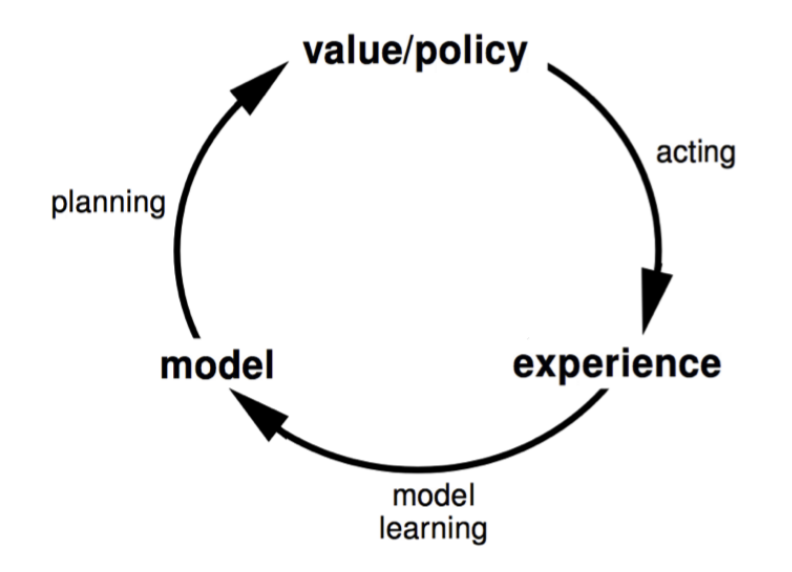
\includegraphics[width=6cm]{model-based-rl}
	\caption{Model-Based RL cycle}
\end{figure}

The advantages of Model-Based RL are that models can be efficiently learned using \textit{supervised learning} methods. It is also possible to then reason of model uncertainty. A disadvantage, however, is that first the model must be learned. Only then can the value function be constructed. This also means there are two sources of approximation error, and the accuracy of the value function is limited to the accuracy of the model.

A \textit{model} $M$ is a representation of an MDP parameterized by $\eta$. In this case, it is assumed that the state and action spaces are known (for simplification). So then, a model $M = (P_\eta, R_\eta)$ represents state transitions $P_\eta \approx P$ and rewards $R_\eta = R$. These can be used to estimate rewards and state transitions:

\begin{equation*}
	\begin{aligned}
		S_{t+1} & \sim P_\eta(S_{t+1} | S_t, A_t)\\
		R_{t+1} & = R_\eta(S_{t+1} | R_t, A_t)
	\end{aligned}
\end{equation*}

Typically, a conditional independence between state transitions and rewards are assumed ($P(S_{t+1}, R_{t+1} | S_t, A_t) = P(S_{t+1} | S_t, A_t)P(R_{t+1} | S_t, A_t)$).

So, the goal is to estimate $M_\eta$ from experience $\{S_1, A_1, R_2, ..., S_T\}$. This is a supervised learning problem. More specifically, it is usually best to split up the two tasks of learning $R_\eta$ and $P_\eta$. $S_t, A_t \Rightarrow R_{t+1}$ is a \textit{regression problem}, while $S_t, A_t \Rightarrow S_{t+1}$ is a \textit{density estimation} problem.

There are a lot of ways to create a model. This chapter focusses on the \textit{Table-Lookup Model}. 

\subsection{Table-Lookup Model}

The idea here is to count the visits $N(s, a)$ to each state-action pair. Then, similar to what TD learns, the idea is to construct the maximum-likelihood Markov model from this. It can be constructed in the following manner.

\begin{equation}
	\begin{aligned}
		& \hat{P^a_{ss'}} = \frac{1}{N(s,a)} \sum_{k = 1}^K \sum_{t = 1}^{T_k} 1(s^k_t, a^k_t, s^k_{t+1} = s, a, s')\\
		& \hat{R^a_{s}} = \frac{1}{N(s,a)} \sum_{k = 1}^K \sum_{t = 1}^{T_k} 1(s^k_t, a^k_t = s, a)r^k_t
	\end{aligned}
	\label{eq:sampling-from-model}
\end{equation}

Alternative, it is possible to record an experience tuple $(S_t, A_t, R_{t+1}, S_{t+1})$ at each time-step $t$. In order to then sample the model, uniformly randomly pick a tuple matching $(S_t, A_t, ., .)$.

\subsection{Planning with a Model}

Given a model $M_\eta = (P_\eta, R_\eta)$, the goal is to solve the MDP $(S, A, P_\eta, R_\eta)$ using a planning algorithm (e.g. Value iteration, Policy iteration, Tree search, ...).

Algorithms like Value iteration are quite expensive, since they go over the entire state(-action) space. \textbf{Sample-Based} planning uses the model to generate samples. This is often much more efficient. It also means more frequent states will be sampled more often. This can be a good property to have.

The sampling happens in the same way as in equation \ref{eq:sampling-from-model}. At each step, model-free RL can be applied to the samples (e.g. Monte-Carlo control, SARSA, Q-Learning, ...).

Given an imperfect model $(P_\eta, R_\eta) \neq (P, R)$, the performance of model-based RL is limited to the optimal policy of approximate MDP $(S, A, P_\eta, R_\eta)$. So, when the model is inaccurate, planning will compute a sub-optimal policy. It is always possible to switch to model-free RL. However, there are ways of reasoning about the \textit{uncertainty} in the model. This can be done using for example Bayesian modelling.


\section{Integrated Architectures}

\begin{figure}[H]
	\centering
	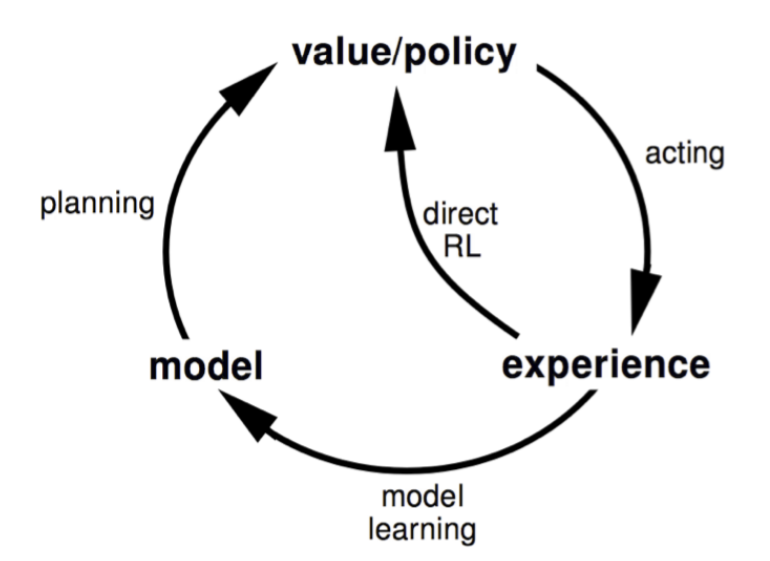
\includegraphics[width=6cm]{dyna}
	\caption{Dyna architecture cycle}
\end{figure}

It is possible to learn and plan the value function (and/or policy) from real and simulated experience. This architecture is referred to as \textbf{Dyna}.The algorithm below uses Dyna with Q-Learning.

\begin{algorithm}[H]
	\caption{Dyna-Q}
	\label{alg:Dyna-Q}
	\begin{algorithmic}
		\REQUIRE $Q$, $M$, $n$ (number of planning steps)
		\STATE $S \Leftarrow$ current state
		\STATE $A \Leftarrow \epsilon$-greedy($S, Q$)
		\STATE Execute $A$; observe $R, S'$
		\STATE $Q(S, A) \Leftarrow Q(S, A) + \alpha \left[R + \gamma \max_a Q(S', a) - Q(S, A)\right]$
		\STATE $M \Leftarrow R,S'$
		\FOR{$i = 1,...,n$}
			\STATE $S, A \Leftarrow$ random previously taken state-action pair
			\STATE $R, S' \Leftarrow M(S, A)$
			\STATE $Q(S, A) \Leftarrow Q(S, A) + \alpha \left[R + \gamma \max_a Q(S', a) - Q(S, A)\right]$
		\ENDFOR
	\end{algorithmic}
\end{algorithm}

Here, the Q-function is learned from both real experience and planned experience.

\section{Simulation-Based Search}

\textbf{Forward search} algorithms select the best action by \textit{lookahead}. They build a search tree with current state $s_t$ at the root. The idea is to use a \textit{model} of the MDP to perform lookahead. Then, only a subsection of the entire MDP must be solved. 

\textbf{Simulation-Based search} simulates episodes of experience from the current state with the model. So, from current state $s_t$, $K$ episodes are sampled:

\begin{equation*}
	\{s_t^k, A_t^k, R_{t+1}^k, ..., S_T^k\}_{k = 1}^K \sim M
\end{equation*}

Then, model-free RL is applied to the simulated episodes. Monte-carlo control gives rise to \textbf{Monte-Carlo search}, while SARSA gives rise to \textbf{TD search}.

Simple Monte-Carlo search uses the mean return to construct Q-values $Q(s_t, a) = \frac{1}{K} \sum_{k = 1}^K G_t$ for each action $a \in A$. This estimates $q_\pi(s_t, a)$, where $\pi$ is the simulation policy. The real action is then taken using $a_t = \arg\max_{a \in A} Q(s_t, a)$.

\subsection{Monte-Carlo Tree Search}

\textbf{Monte-Carlo Tree Search} (MCTS) works differently. It has two policies, a \textit{Tree policy} and a \textit{Default policy}. The tree policy picks the actions to maximize $Q(S, A)$ and the default policy is fixed and takes random actions. So, the tree policy improves over time.

At each simulation, it first uses the tree policy to find with state to simulate from. Then, the simulation (also referred to as rollout) happens using the default policy. The Q-values are then the mean return of episodes.

\begin{equation*}
	Q(s, a) = \frac{1}{N(s, a)} \sum^K_{k = 1} \sum^T_{u = t} 1(S_u, A_u = s, a)G_u
\end{equation*}

After the planning has finished, the real action is again taken using policy $a_t = \arg\max_{a \in A} Q(s_t, a)$. MCTS is MC-control applied to simulated experience. It converges on the optimal search tree, $Q(S, A)$ becomes $q_*(S, A)$.

There are several advantages to using MCTS
\begin{itemize}
	\item The best-first search is highly selective
	\item Evaluates states dynamically, unlike DP
	\item The use of sampling breaks the curse of dimensionality
	\item It works for black-box models, all it needs are samples
	\item Computationally efficient, anytime and parallelisable
\end{itemize}

\subsection{Temporal-Difference Search}

The idea is to use TD instead of MC, by bootstrapping. It applies SARSA to the sub-MDP. It can be helpful for the following reasons
\begin{itemize}
	\item TD search reduces variance, but increases bias
	\item TD search is usually more efficient than MC search
	\item TD($\lambda$) can be much more efficient than MC search
\end{itemize}

\textbf{TD search} simulates episodes from the current state $s_t$. It estimates the value function $Q(S, A)$. At each step of the simulation, $\Delta Q(S, A) = \alpha (R + \gamma Q(S', A') - Q(S, A))$. Actions are selection $\epsilon$-greedily with respect to the Q-values. A function approximator can also be used for Q.

There is another idea called \textbf{Dyna-2}. The agent stores two sets of feature weights: \textit{Long-term memory} and \textit{Short-term (working) memory}. 

The long-term memory is updated from real experience with the environment. It is perceived as general knowledge that applies to any episode. On the other hand, the short-term memory is updated from simulated experience using TD search. This can figure out specific local knowledge about the current situation.

The value function is then a sum of the long- and short-term memories.

\let\cleardoublepage\clearpage
\chapter{Exploration and Exploitation}

The trade-off between exploration and exploitation is a fundamental problem in Reinforcement Learning and online decision-making. It provides a trade-off between making a decision based on the current beliefs, or gather more of this information.

In general, the long-term is preferred over short-turn. This means the best strategy might include short-term sacrifices. The foal is to gather enough information to make the best overall decisions.

This chapter will first explain exploration in a special forms of an MDP, called bandit problems. Finally, these ideas are generalized to the general MDP.

There are lots of \textit{principles} to make sure to explore. There include but are not limited to the following
\begin{itemize}
	\item \textbf{Naive Exploration}: Add noise to greedy policy (e.g. $\epsilon$-greedy)
	\item \textbf{Optimistic Initialization}: Assume the best until proven otherwise
	\item \textbf{Optimism in the face of uncertainty}: Prefer actions with uncertain values
	\item \textbf{Probability Matching}: Select actions based on probability their are best
	\item \textbf{Information State Search}: Look-ahead search incorporating value of information
\end{itemize}

\section{Multi-Armed Bandits}

A multi-armed bandit is a tuple $(A, R)$. Here, $A$ is a known set of actions (arms) and $R^a(r) = \Prob\left[r | a\right]$ is an unknown probability distribution over rewards. At each step $t$, the agent chooses an action $a_t \in A$. Then, the environment generates a reward $r_t \sim R^{a_t}$. The goal is to maximize the cumulative reward $\sum_{T = 1}^{t} r_T$.

The goal is to maximize this reward. However, this can otherwise be states as \textit{minimizing} the total \textbf{regret}. The action-value is the expected reward of an action ($Q(a) = \E\left[r | a\right]$). The optimal value $V* = Q(a^*) = \max_{a \in A} Q(a)$.

The regret is the measured opportunity loss for one step: $l_t = \E\left[V^* - Q(a_t)\right]$. The \textit{total regret} is then equal to the total opportunity loss $L_t = \E\left[\sum_{T = 1}^{t} V^* - Q(a_t)\right]$.

It is possible to count regret. The \textit{count} $N_t(a)$ is the expected number of selection for action $a$. For that action, there is a \textit{gap} in difference of value between $a$ and $a^*$. This gap equals $\Delta_a = V^* - Q(a)$. The regret can then be rewritten to the following
\begin{equation*}
	\begin{aligned}
		L_t & = \E\left[\sum_{T = 1}^{t} V^* - Q(a_t)\right]\\
		    & = \sum_{a \in A} \E\left[N_t(a)\right] (V^* - Q(a_t))\\
		    & = \sum_{a \in A} \E\left[N_t(a)\right] \Delta_a
	\end{aligned}
\end{equation*}

So, the regret is a function of the gaps and counts. A good algorithm will ensure small counts for large gaps. There is a problem however; the gaps are not known.

\begin{figure}[H]
	\centering
	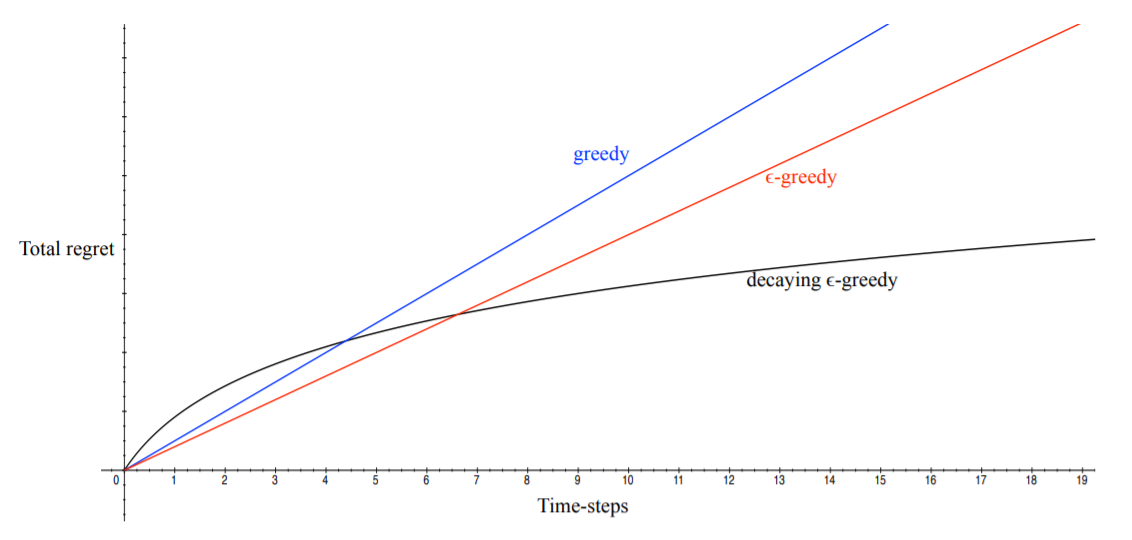
\includegraphics[width=10cm]{regret-over-time}
	\caption{Total regret over time}
	\label{fig:regret-over-time}
\end{figure}

From \ref{fig:regret-over-time}, the following observations can be made. If an algorithm \textit{never}- or \textit{forever} explores, the total regret will be \textit{linear}. This is not good, since the goal is to minimize regret while exploring. The idea of \textit{decaying} $\epsilon$-greedy is interesting, since it will converge to a logarithmic regret.

Lets estimate $Q(a) \approx \hat{Q}_t(a)$. The value of each action can be evaluated by MC-evaluation: $\hat{Q}_t(a) = \frac{1}{N_t(a)} \sum_{t = 1}^{T} r_t 1(a_t = a)$.

Since the \textit{greedy} algorithm always selects the action with the highest value, it can lock onto a sub-optimal action forever, thus receiving a linear total regret.

Using an \textit{$\epsilon$-greedy} algorithm, the constant $\epsilon$ ensures that the minimum regret $l_t \geq \frac{\epsilon}{A} \sum_{a \in A} \Delta_a$. Thus, the total regret is also linear.

A simple but powerful idea is to use \textbf{Optimistic Initialization}. Initialize $Q(a)$ to a very high value and from there on update the action-value by MC evaluation starting with $N(a) > 0$. It encourages exploration early on, but can still lock onto sub-optimal actions. In practice however, this generally works really well.

The \textit{decaying $\epsilon$-greedy} algorithm works by picking a decaying schedule for $\epsilon_1, \epsilon_2, ...$. Imagine the following schedule
\begin{equation*}[
	\begin{aligned}
		c & > 0\\
		d & = \min_{a | \Delta_a > 0} \Delta_i\\
		\epsilon_t & = \min \{1, \frac{c|A|}{d^2t}\}
	\end{aligned}
\end{equation*}

There is a problem with the schedule though. It uses advance knowledge about gaps. So, the goal is to find an algorithm with sub-linear regret for any multi-armed bandit without using knowledge of $R$.

The performance of any algorithm is determined by the \textit{similarity} between the optimal arm and other arms. Hard problem have similar-looking arms with different means. This can be described as the size of the gap, and the similarity in distributions (measure by KL-divergence).

The following \textbf{Lower Bound} is a theorem. It means the \textit{asymptotic total regret is at least logarithmic in the number of steps}.

\begin{equation*}
	\lim_{t \rightarrow \infty} L_t \geq \log t \sum_{a | \Delta_a > 0} \frac{\Delta_a}{KL(R^a||R^{a^*})}
\end{equation*}

\subsection{Upper Confidence Bounds}

\begin{figure}[H]
	\centering
	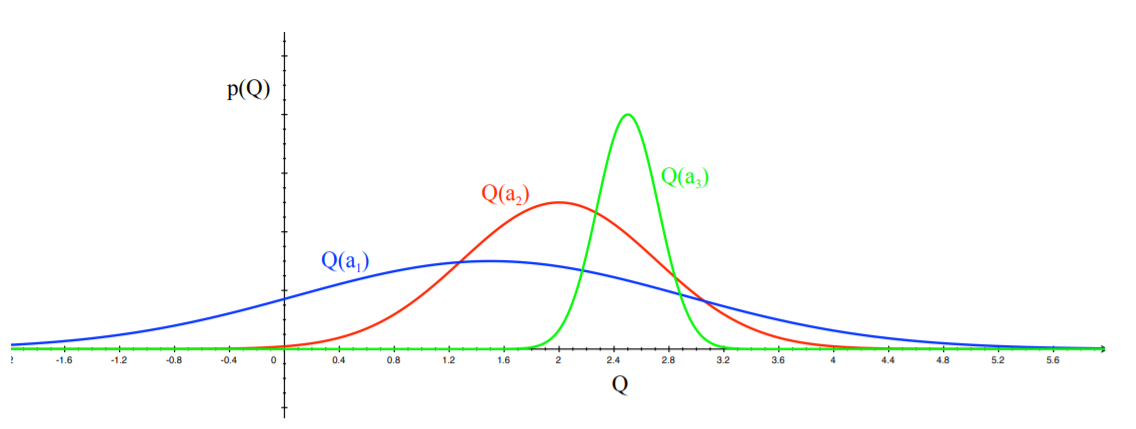
\includegraphics[width=10cm]{oitfou-before}
\end{figure}

Take a look at the figure above. The idea of \textbf{Optimism in the Face of Uncertainty} is to pick the action with the highest potential. This would be $a_1$, since the tail of the distribution is the best one of them all. Say you pick this action. Then, the distribution gets updated.

\begin{figure}[H]
	\centering
	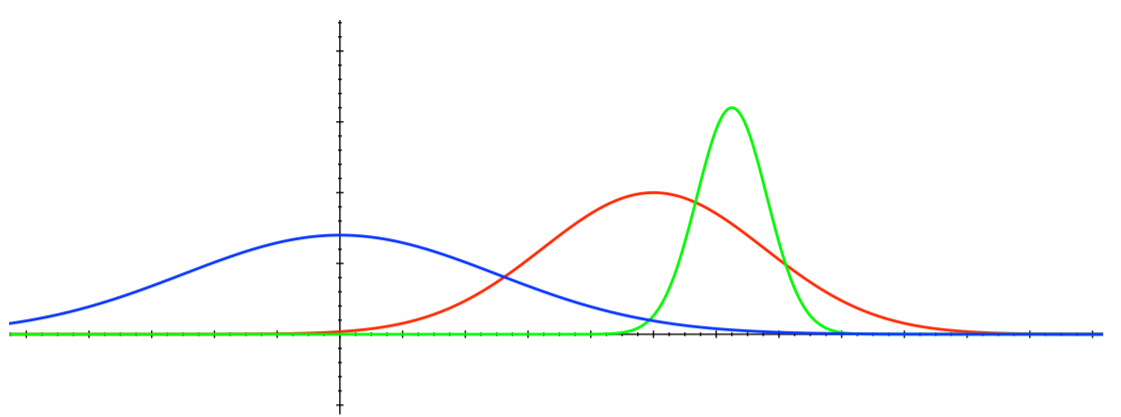
\includegraphics[width=10cm]{oitfou-after}
\end{figure}

Now, we are more certain about the actual value of $Q(a_1)$ and thus more likely to pick another action until the optimal one has been discovered.

Another way to estimate uncertainty is through \textbf{Upper Confidence Bounds} (UCB). An upper confidence $\hat{U}_t(a)$ can be calculated for each action-value, such that $Q(a) \leq \hat{Q}_t(a) + \hat{U}_t(a)$ with high probability. The action maximizing the UCB is then selected.

By \textbf{Hoeffding's Inequality}, $\Prob\left[\E\left[X\right] > \bar{X}_t + u\right] \leq e^{-2tu^2}$ for $\bar{X}_t = \frac{1}{T} \sum_{t = 1}^T X_t$, where $X_t$ is an i.i.d. r.v. in $[0, 1]$. When applying this to the bandit problem, the following can be derived

\begin{equation*}
	\Prob\left[Q(a) > \hat{Q}_t(a) + U_t(a)\right] \leq e^{-2N_t(a)U_t(a)^2}
\end{equation*}

Now, pick a probability $p$ that the true value exceeds the UCB.

\begin{equation*}
	\begin{aligned}
		p & = e^{-2N_t(a)U_t(a)^2}\\
		U_t(a) & = \sqrt{\frac{-\log p}{2 N_t(a)}}
	\end{aligned}
\end{equation*}

Since the goal is to reduce the probability as more rewards are observed, set e.g. $p = t^{-4}$. Then ensures the optimal action is selected when $t \rightarrow \infty$. The final equation becomes

\begin{equation*}
	U_t(a) = \sqrt{\frac{2 \log t}{N_t(a)}}
\end{equation*}

This leads to the \textbf{UCB1} algorithm

\begin{equation*}
	a_t = \arg\max_{a \in A} Q(a) + \sqrt{\frac{2 \log t}{N_t(a)}}
\end{equation*}

\textit{Theorem}: the UCB algorithm achieves logarithmic asymptotic total regret
\begin{equation*}
	\lim_{t \rightarrow \infty} L_t \leq 8 \log t \sum_{a | \Delta_a > 0} \Delta_a
\end{equation*}

\subsection{Bayesian Bandits}

So far, no assumptions were made about the reward distribution $R$, except for bounds on rewards. \textbf{Bayesian Bandits} exploit prior knowledge of rewards, $p\left[R\right]$. They compute the posterior distribution of reward $p\left[R | h_t\right]$, where $h_t = a_1, r_1, ..., a_{t-1}, r_{t-1}$ is the history. The posterior distribution can then be used to guide exploration.

The following is an example. Assume that the reward distribution is Gaussian, so $R_a(r) = N(r; \mu_a, \sigma_a^2)$. The Gaussian posterior over $\mu_a$ and $\sigma_a^2$ can be computed using Bayes' law: $p[\mu_a, \sigma_a^2; h_t] \propto p[\mu_a, \sigma_a^2] \prod_{t | a_t = a} N(r_t; \mu_a, \sigma_a^2)$.

Then, pick the action that maximizes the standard deviation of $Q(a)$, so $a_t = \arg\max_{a \in A} \mu_a + \frac{c \sigma_a}{\sqrt{N(a)}}$. This is a Bayesian way to compute Upper Confidence Bounds.

\begin{figure}[H]
	\centering
	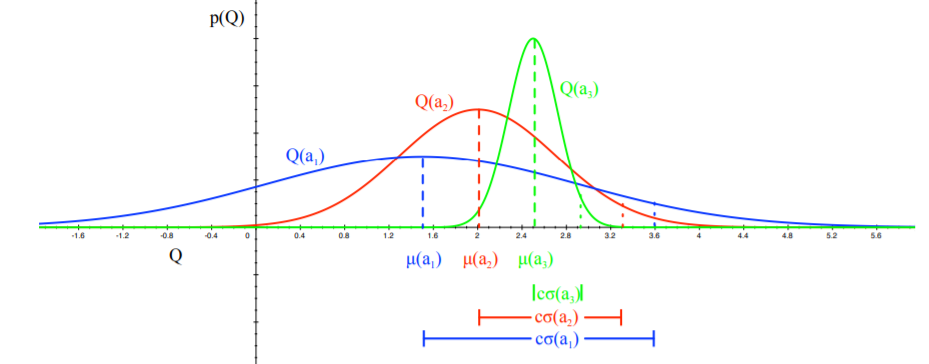
\includegraphics[width=10cm]{ucb-bayesian}
\end{figure}

Here, the blue action would be taken. This is because the mean and standard deviation summed up is the largest (assuming an equal number of visits).

\subsection{Probability Matching}

\textbf{Probability Matching} selects an action $a$ according to the probability that $a$ is optimal. It can be calculated using
\begin{equation*}
	\pi(a) = \Prob \left[Q(a) = \max_{a'} Q(a') | R_1, ..., R_{t-1}\right]
\end{equation*}
This concept is optimistic in the face of uncertainty, since uncertain actions have a higher probability of being the maximum. A disadvantage however is that it can be difficult to be computed analytically from the posterior.

\textbf{Thompson Sampling} is sample-based probability matching. The policy can be computed using
\begin{equation*}
	\pi(a) = \E\left[1(Q(a) = \max_{a'} Q(a')) | R_1, ..., R_{t-1}\right]
\end{equation*} 
Then, use Bayes' law to compute the posterior distribution $P_w(Q|R_1, ..., R_{t-1})$. First sample an action-value $Q(a)$ from the posterior. Then, choose action $A_t = \arg\max_{a \in A} Q(a)$.

\subsection{Information State Search}

The goal of exploration is to gain more information about the environment. If it is possible to quantify how much this information is worth. When this value is known, the optimal trade-off between exploration and exploitation is known.

The idea is to look at bandits as \textit{sequential} decision-making processes instead of \textit{one-step}. At each step, there is an \textbf{information state} $\bar{s} = f(h_t)$. So, the state is a summary of all history that has been accumulated so far. Each action $a$ then causes a transition to a new information state $\bar{s}'$, with probability $\bar{P}^a_{\bar{s}\bar{s}'}$.

This defines the MDP $\bar{M}$ in augmented information state space $\bar{M} = (\bar{S}, A, \bar{P}, R, \gamma)$.

An example of this are Bernoulli Bandits, so lets say $R^a = Bernoulli(\mu_a)$. The goal is to find the arm with the highest $\mu_a$. The information state space $\bar{s} = (\alpha, \beta)$, where $\alpha_a$ and $\beta_b$ count when the reward was 0 or 1 respectively.	 This MDP can then be solved by previously discussed Reinforcement Learning algorithms. There is an alternative approach, referred to as \textbf{Bayes-adaptive RL}. For Bernoulli bandits, it finds the Bayes-optimal exploration/exploitation trade-off with respect to the prior distribution.

Imagine a problem of drug assignment. There are two drugs 1 and 2 that can be used; $\bar{s} = (\alpha_1, \beta_1, \alpha_2, \beta_2)$. First, start with a $Beta(\alpha_a, \beta_a)$ prior over reward function $R^a$. Each time $a$ is selected, the distribution gets updated accordingly, since a success will increase beta, and a failure increases alpha. Here, each state transition corresponds to a Bayesian model update. 

The solution of this problem is known as the \textit{Gittens} index, and can be computed by solving the MDP (by using for example MCTS for planning).

\section{Contextual Bandits}

A \textbf{Contextual Bandit} is a tuple $(A, S, R)$. Instead of the bandit problem, there is now also a state space, which provides \textit{context} to the problem. $S = \Prob[s]$ is an unknown distribution over the contexts. Then, the reward $R^a_s(r) = \Prob[r|s, a]$ is an unknown probability distribution of the rewards. At each time step, the environment generates $s_t \sim S$. Then, an agent selects $a_t \in A$, to which the environment generates $r_t \sim R^{a_t}_{s_t}$. The goal is to maximize $\sum_{T=1}^t r_T$.

This section explains the concept of \textbf{Linear UCB}. The action-value function needs to be estimated: $Q(s, a) = \E[r|s,a] \approx Q_\theta(s, a) = x(s, a)^\intercal \theta$. The parameters of this linear function can be estimated by least-squares. The solution is
\begin{equation*}
	\theta_t = \left(\sum_{T=1}^t x(s_T, a_T)x(s_T, a_T)^\intercal\right)^{-1} \sum_{T=1}^t x(s_T, a_T)r_T
\end{equation*}

Least squares regression estimates $Q_\theta(s, a)$. However, it can also be used to estimate the variance of the action-value $\sigma^2_\theta(s, a)$. The idea is to add a bonus for uncertainty, $U_\theta(s, a) = c\sigma$, where the UCB is the number of standard deviations above the mean defined by $c$.

For least squares regression, parameter covariance is $A^{-1} = \left(\sum_{T=1}^t x(s_T, a_T)x(s_T, a_T)^\intercal\right)^{-1}$. The action-value is linear in features, so

\begin{equation*}
	\begin{aligned}
		\sigma^2_\theta(s, a) & = x(s, a)^\intercal A^{-1} x(s, a)\\
		a_t & = \arg\max_{a \in A} Q_\theta(s_t, a) + c\sigma_\theta(s_t, a)\\
		a_t & = \arg\max_{a \in A} Q_\theta(s_t, a) + c \sqrt{x(s, a)^\intercal A^{-1} x(s, a)}
	\end{aligned}
\end{equation*}

\section{MDPs}

All previously described principles for exploration/exploitation can apply to MDPs with slights modifications.

\begin{itemize}
	\item Optimistic Initialization
	\begin{itemize}
		\item Model-Free RL
		
		The idea is to initialize $Q(s, a)$ to $\frac{r_{max}}{1 - \gamma}$. This encourages systematic exploration of states and actions.
		\item Model-Based RL
		
		Here, an optimistic model of the MDP is constructed. For example, transitions to a terminal state are initialized with $r_{max}$ reward. An example is the RMax algorithm (Brafman and Tennenholtz).
	\end{itemize}

	\item Optimism in the Face of Uncertainty
		\begin{itemize}
		\item Model-Free RL
		
		The goal is to maximize UCB on the action-value function $Q^\pi(s, a)$. $a_t = \arg\max_{a \in A} Q(s_t, a) + U(s_t, a)$. It estimates uncertainty in policy evaluation. However, it completely ignores uncertainty in the policy improvement step.
		
		For this reason, maximize UCB on $Q^*(s, a)$ instead. $a_t = \arg\max_{a \in A} Q(s_t, a) + U_1(s_t, a) + U_2(s_t, a)$. This estimates uncertainty in both policy evaluation and policy improvement. However, estimating policy improvement uncertainty is hard to do.		
		
 		\item Model-Based RL
		
		Bayesian Model-Based RL maintains a posterior distribution over MDP models. Both transitions and rewards are estimated $p[P, R| h_t], h_t = s_1, a_1, r_2, ..., s_t$. This posterior can then be used to guide exploration by for example Bayesian UCB or Thompson Sampling.
	\end{itemize}

	\item Probability Matching
	
	Thompson sampling implements probability matching
	\begin{equation*}
		\begin{aligned}
			\pi(s, a | h_t) & = \Prob[Q^*(s, a) > Q^*(s, a'), \forall a' \neq a | h_t]\\
							& = \E_{P, R| h_t}\left[1(a = \arg\max_{a \in A} Q^*(s, a))\right]
		\end{aligned}
	\end{equation*}

	Bayes' Law can be used to compute posterior distribution $p[P, R| h_t]$. Then, sample an MDP $P, R$ from the posterior. Then, solve this MDP using a favored planning algorithm to obtain $Q^*(s, a)$. Then, select the optimal action from the sample MDP by $a_t \arg\max_{a \in A} Q^*(s_t, a)$. 
		
	\item Information State Search
	
	MDPs can also be augmented to include an information state. The augmented state becomes $(s, \hat{s})$, where $s$ is the original state within the MDP, and $\hat{s}$ is accumulated information about the history. Each action $a$ causes a transition to $s'$ with probability $P^a_{ss'}$. However, a new information state $\hat{s}'$ is also created.
	
	The posterior distribution over the MDP model is an information state $\hat{s_t} = \Prob[P, R| h_t]$. An augmented MDP over $(s, \hat{s})$ is called a \textbf{Bayes-Adaptive MDP}.
	
	Solving this MDP gives rise to the optimal exploration/exploitation trade-off. However, the Bayes-Adaptive MDP is typically enormous. Simulation-based search has been proven effective to this problem.
\end{itemize}
\let\cleardoublepage\clearpage
\chapter{RL in Classic Games}

Why are classic games such a meaningful area to apply Reinforcement Learning to? The main point is that these games usually have quite simple rules, but very deep concepts. They also provide for a meaningful IQ test, and encapsulate real world issues. This makes it a really interesting field for Reinforcement Learning.

\section{Game Theory}

In order to get a sense of optimality in multiplayer games, the field of Game Theory is often used. The aim is to find the optimal policy $\pi^i$ for the $i$-th player. If all other players fix their policies ($\pi^{-i}$), the \textbf{best response} $\pi_*^i(\pi^{-i})$ is the optimal policy against those policies.

There is a problem with this, because it basically learns the optimal policy for \textit{one} fixed policy of the opponents. Instead, the goal is to find the optimal policy against all policies opponents can have. The most well-known solution to this is referred to as the \textbf{Nash equilibrium}. This is a joint policy for all players.

\begin{equation*}
	\pi^i = \pi_*^i(\pi^{-i})
\end{equation*}

Here, every player's policy is a best response. This means no player would choose to deviate from this equilibrium.

\begin{itemize}
	\item Best Response is a solution of a single-agent RL problem.
	
	Other players become part of the environment, and the game is reduced to an MDP. The best response is then an optimal policy of this MDP.
	
	\item Nash equilibrium is a fixed-point of self-play RL
	
	Experience is generated by playing games between agents $a_1 \sim \pi^1, a_2 \sim \pi^2, ...$. Each agent learns the best response to other players. One player's policy determines another player's environment. This means all players are adapting to each other.
\end{itemize}

To keep things relatively simple, this chapter restricts itself to \textbf{two player}, \textbf{zero sum} games. Zero sum games have equal and opposite rewards $R^1 + R^2 = 0$. Methods for finding Nash equilibria in these games are discussed.

\section{Minimax Search}

In these types of games, the value function defines the expected total reward given joint policies $(\pi^1, \pi^2)$
\begin{equation*}
	v_\pi(s) = \E_\pi[G_t | S_t = s]
\end{equation*}

A \textit{minimax} value function maximizes player 1's expected return while minimizing the one from player 2. The optimal value function becomes
\begin{equation*}
	v_*(s) = \max_{\pi^1} \min_{\pi^2} v_\pi(s)
\end{equation*}

A \textit{minimax} policy $(\pi^1, \pi^2)$ is a joint policy which achieves the minimax values. For two-player zero sum games, there exists a unique minimax value function. In this case, a minimax policy is a Nash equilibrium.

There is a problem though. The search tree grown exponentially at every level. This means it is impractical to search all the way to the end of the game. A simple solution to this problem uses a value function approximation $v(s, w) \approx v_\pi(s)$ at the leaf nodes of the search tree. Then, it is possible to run minimax to some fixed depth with respect to the leaf values.

\section{Self-Play RL}

Similar to this fixed function approximation in the last section, it is possible to apply value-based RL algorithms to games of self-play. Any algorithm like $MC, TD(0), TD(\lambda), ...$ can be used. For deterministic games, it is sufficient to estimate $v_*(s)$. The idea uses the following short proof
\begin{equation*}
	\begin{aligned}
		q_*(s, a) & = \sum_{s'} P^a_{ss'} v_*(s)\\
		q_*(s, a) & = v_*(s')
	\end{aligned}
\end{equation*}

Actions are selected by min- or maximizing the value of the next state
\begin{equation*}
	\begin{aligned}
		A_t & = \arg\max_a v_*(S_t') \text{ for the maximizing player}\\
		A_t & = \arg\min_a v_*(S_t') \text{ for the minimizing player}
	\end{aligned}
\end{equation*}

This improves the joint policy for both players.

\section{Combining RL and Minimax Search}

The ideas of both these methods can be combined. This section focuses on some ideas to combine both.

\subsection{Simple TD}

As previously seen, the idea of TD is to update the value function towards the successor value. The idea of \textit{Simple TD} is to first learn the value function in TD learning. After learning, this value function can be used in minimax search (without any learning). 
\begin{equation*}
	v_+(S_t, w) = minimax_{s \in leaves(S_t)} v(s, w)
\end{equation*}

An important question arises when using this approach: can the value function be learning directly from minimax search values? This could increase performance more quickly, since it can be hard to find a terminal state without search.

\subsection{TD Root}

The idea of \textit{TD Root} is to update the value towards the successor search value. Imagine the tree is at root node $S_t$. After taking an action, $S_{t+1}$ is explored next. TD would update the value of $S_t$ towards the value of $S_{t+1}$. The value of $S_{t+1}$ equals the value of the minimax search backup, so $v(S_{t+1}, w) = v(l(S_{t+1}), w)$, where $l(s)$ is the leaf node achieving minimax value from $s$.

This was actually the first ever TD learning algorithm applied to a checkers program that learned by self-play. It was able to defeat an amateur human player. This algorithm was then used and extended to perform better.

\subsection{TD Leaf}

One idea is to think about the whole search. Instead of updating the value of $S_t$, the value of the leaf $l(S_t)$ should be updated. This is the case, because that is the node that contributed to the minimax value $v(S_t)$. This results in the back-up $v(l(S_t), w) \leftarrow v(l(S_{t+1}), w)$, instead of $v(S_t, w) \leftarrow v(l(S_{t+1}), w)$ as seen in TD Root.

\textit{Knightcap} used TD leaf in chess. It started by only knowing standard piece values, and learned weights using TD leaf. The search used $\alpha\beta$-pruning to speed up the minimax search. It ended up achieving master-level play after a small number of games. However, it was not effective in self-play or without starting from good weights. In checkers however, a similar algorithm called Chinook was able to play at superhuman level.

\subsection{TreeStrap}

There is still something to optimize. The previously algorithms use the values obtained from the minimax search only once. \textit{TreeStrap} updates search values towards deeper search values. Minimax search values are computed at \textit{all} nodes in the search. The backup $\forall s \in nodes(S_t): v(s, w) \leftarrow v(l(s), w)$ is performed.

\textit{Meep}, a chess algorithm using TreeStrap, was able to beat 13/15 international masters starting from random initial weights. It is both effective in self-play and random initial weights.

\subsection{Simulation-Based Search}

As you have seen now, self-play reinforcement learning can replace search. Next to the idea of minimax, it is also possible to simulate games of self-play from root state $S_t$, and then apply RL to this simulated experience.

Previously, a concept using Monte-Carlo Control called \textit{MCTS} was discussed. The most effective variant of this search uses the UCT-algorithm to guide exploration/exploitation in every node. It actually turns out self-play UCT converges on minimax values in zero-sum, 2-player games.

\section{RL in Imperfect-Information Games}

In imperfect information games, players have different information states and therefore separate search trees. In this tree, there is one node for each information state. These nodes summarize what a player knows (e.g. the cards they have seen).

There may be many real states that share the same information state, but there may also be aggregate states (e.g. those with a similar value).

There are multiple ways to solve for these information-state game trees.
\begin{itemize}
	\item Iterative forward-search methods 
	
	An example of this is Counterfactual Regret Minimization
	\item Self-play Reinforcement learning
	
	Here, a variant of MCTS, called Smooth UCT is discussed briefly. Applying the method to the game of Poker resulted in 3 silver medals in two- and three-player Poker. It outperformed massive-scale forward-search agents.
\end{itemize}

\subsection{Smooth UCT}

Using Monte-Carlo Tree Search in fully observable games has shown promising. However, improvements must be made to let it perform well in imperfect information games. In Poker for example, naive MCTS diverges, since its approach is just not well-fitted for these types of games.

However, a variant of UCT, inspired by a game-theoretic concept called \textbf{Fictitious Player} was implemented. The idea is that the agent learns against and to respond to opponents' \textit{average} behavior. This gives a much robust approach.

The average strategy can be extracted from nodes' action counts, $\pi_{avg}(a | s) = \frac{N(s, a)}{N(s)}$. Then, at each node, pick actions according to
\begin{equation*}
	A \sim \begin{cases}
		UCT(S), & \text{ with probability } \epsilon\\
		\pi_{avg}(.|S), & \text{ with probability } 1 - \epsilon
	\end{cases}
\end{equation*}

Empirically, in variants of Poker, smooth UCT converged to the Nash equilibrium while naive MCTS diverged.


\let\cleardoublepage\clearpage

\backmatter
\bibliographystyle{named}
\bibliography{./TeX_files/bibliography}
% bibliography, glossary and index would go here.

\end{document}